% Converted from reference/DB4OFlare (MadCap Flare, Java target)

\chapter{Configuration}
\label{ref:configuration}

db4o is configured by its configuration API. The configuration allows you to adjust db4o to your scenarios.

\section*{Configure db4o}

In order to configure db4o, you need to create a new configuration-instance and set the desired settings on it. After that, you pass the configuration-instance to the object-container factory.

Note that you cannot share a configuration-instance. For each object-container you create, you need to pass in a new configuration-instance. It's recommended to create a method which will return a new configuration instance on request:

\section*{Embedded-Configuration}

For an embedded container you can configure the \hyperref[ref:configuration-common-configuration]{common} (p.~\pageref{ref:configuration-common-configuration})-, \hyperref[ref:configuration-file-configuration]{file} (p.~\pageref{ref:configuration-file-configuration})- and \hyperref[ref:configuration-id-system]{id-system} (p.~\pageref{ref:configuration-id-system})-configuration.

\begin{lstlisting}
EmbeddedConfiguration configuration = Db4oEmbedded.newConfiguration();
// change the configuration...
ObjectContainer container = Db4oEmbedded.openFile(configuration, "database.db4o");
\end{lstlisting}

\section*{Server-Configuration}

For an server you can configure the \hyperref[ref:configuration-common-configuration]{common} (p.~\pageref{ref:configuration-common-configuration})-, \hyperref[ref:configuration-file-configuration]{file} (p.~\pageref{ref:configuration-file-configuration})-, \hyperref[ref:configuration-network-configuration]{networking} (p.~\pageref{ref:configuration-network-configuration})-, \hyperref[ref:configuration-server-configuration]{server} (p.~\pageref{ref:configuration-server-configuration})- and \hyperref[ref:configuration-id-system]{id-system} (p.~\pageref{ref:configuration-id-system})-configuration.

\begin{lstlisting}
ServerConfiguration configuration = Db4oClientServer.newServerConfiguration();
// change the configuration...
ObjectServer server = Db4oClientServer.openServer(configuration, "database.db4o", 1337);
\end{lstlisting}

\section*{Client-Configuration}

For an client you can configure the \hyperref[ref:configuration-common-configuration]{common} (p.~\pageref{ref:configuration-common-configuration})-, \hyperref[ref:configuration-network-configuration]{networking} (p.~\pageref{ref:configuration-network-configuration})-, \hyperref[ref:configuration-client-configuration]{client} (p.~\pageref{ref:configuration-client-configuration})- and \hyperref[ref:configuration-id-system]{id-system} (p.~\pageref{ref:configuration-id-system})-configuration.

\begin{lstlisting}
ClientConfiguration configuration = Db4oClientServer.newClientConfiguration();
// change the configuration...
ObjectContainer container = Db4oClientServer.openClient(configuration, "localhost", 1337, "user", "pwd");
\end{lstlisting}

\section*{Configuration Is Not Persistent}

The db4o configuration is not persistent with a few exception. This means that you need to configure db4o each time you create a object-container instance.

\section*{Configuration in Client/Server-Mode}

For using db4o in client/server mode it is recommended to use the same configuration on the server and on the client. To set this up nicely it makes sense to create one application class with one method that returns the required configuration and to deploy this class both to the server and to all clients.

\section*{Configuration-Settings Overview}

The configuration-settings which are common across -client, embedded and db4o-server are summed up here: \hyperref[ref:configuration-common-configuration]{See "Common Configuration"} (p.~\pageref{ref:configuration-common-configuration})

\section{Common Configuration}
\label{ref:configuration-common-configuration}

The common-configuration applies to the embedded-, client- and the server-mode of db4o. All the common configuration is accessible via the common-getter on the configuration-object.

\subsection*{Overview}

Here's a overview over all common configuration-settings which you can change:

{\small
\begin{longtable}{|p{\dimexpr(\linewidth-4\arrayrulewidth)*1/3-2\tabcolsep\relax}|p{\dimexpr(\linewidth-4\arrayrulewidth)*1/3-2\tabcolsep\relax}|p{\dimexpr(\linewidth-4\arrayrulewidth)*1/3-2\tabcolsep\relax}|}
\hline
 & Same in C/S\footnote{This setting needs to be the same on the server and all clients.} & Can not change \footnote{This setting has to be set the first time when the database is created. You cannot change is for an existing database.} \\ \hline
\textbf{\hyperref[ref:configuration-common-activation-depth]{ActivationDepth} (p.~\pageref{ref:configuration-common-activation-depth})}: Change globally the activation-depth. &  &  \\ \hline
\textbf{\hyperref[ref:configuration-common-alias]{Aliases} (p.~\pageref{ref:configuration-common-alias})}: Configure aliases for class and package-names. &  &  \\ \hline
\textbf{\hyperref[ref:configuration-common-updating-db4o-file-format]{AllowVersionUpdates} (p.~\pageref{ref:configuration-common-updating-db4o-file-format})}: Allow/Disallow to update the database-format. & Yes &  \\ \hline
\textbf{\hyperref[ref:configuration-common-automatic-shutdown]{AutomaticShutDown} (p.~\pageref{ref:configuration-common-automatic-shutdown})}: Close the database when the application exits. &  &  \\ \hline
\textbf{\hyperref[ref:configuration-common-btree-node-size]{BTreeNodeSize} (p.~\pageref{ref:configuration-common-btree-node-size})}: Tune the size of the B-tree-node which are used for the indexes. &  &  \\ \hline
\textbf{\hyperref[ref:configuration-common-no-callbacks]{Callbacks} (p.~\pageref{ref:configuration-common-no-callbacks})}: Turn object-callbacks on an off. &  &  \\ \hline
\textbf{\hyperref[ref:configuration-common-calling-constructors]{CallConstructors} (p.~\pageref{ref:configuration-common-calling-constructors})}: Use or bypass the constructor for creating objects. &  &  \\ \hline
\textbf{\hyperref[ref:configuration-common-no-schema-changes]{DetectSchemaChanges} (p.~\pageref{ref:configuration-common-no-schema-changes})}: Disable/Enable schema changes detection. &  &  \\ \hline
\textbf{\hyperref[ref:configuration-common-diagnostics]{Diagnostic} (p.~\pageref{ref:configuration-common-diagnostics})}: Add diagnostic-listeners. &  &  \\ \hline
\textbf{\hyperref[ref:configuration-common-exceptionsonnotstorable]{ExceptionsOnNotStorable} (p.~\pageref{ref:configuration-common-exceptionsonnotstorable})}: Enable/Disable exceptions on not storable objects. &  &  \\ \hline
\textbf{\hyperref[ref:configuration-common-intern-strings]{InternStrings} (p.~\pageref{ref:configuration-common-intern-strings})}: Will call the intern-method on the retrieved strings. &  &  \\ \hline
\textbf{\hyperref[ref:configuration-common-mark-transient]{MarkTransient} (p.~\pageref{ref:configuration-common-mark-transient})}: Configure a Annotation for marking fields as transient. &  &  \\ \hline
\textbf{\hyperref[ref:configuration-common-message-level]{MessageLevel} (p.~\pageref{ref:configuration-common-message-level})}: Configure the logging-message level. &  &  \\ \hline
\textbf{\hyperref[ref:configuration-common-name-provider]{NameProvider} (p.~\pageref{ref:configuration-common-name-provider})}: Configure the toString() value of the object-container. &  &  \\ \hline
\textbf{\hyperref[ref:configuration-common-max-stack-size]{MaxStackSize} (p.~\pageref{ref:configuration-common-max-stack-size})}: Configure how many recursive operations are executed directly on the stack. &  &  \\ \hline
\textbf{\hyperref[ref:configuration-objectclass-configuration]{ObjectClass} (p.~\pageref{ref:configuration-objectclass-configuration})}: Configure class-specific settings. &  &  \\ \hline
\textbf{\hyperref[ref:configuration-common-disable-optimize-nq]{OptimizeNativeQueries} (p.~\pageref{ref:configuration-common-disable-optimize-nq})}: Enable runtime query optimization. &  &  \\ \hline
\textbf{\hyperref[ref:configuration-common-out-stream]{OutStream} (p.~\pageref{ref:configuration-common-out-stream})}: Configure the log message output stream &  &  \\ \hline
\textbf{\hyperref[ref:configuration-common-query-modes]{Queries} (p.~\pageref{ref:configuration-common-query-modes})}: Configure query behaviors &  &  \\ \hline
\textbf{\hyperref[ref:advanced-topics-db4o-reflection-api]{ReflectWith} (p.~\pageref{ref:advanced-topics-db4o-reflection-api})}: Configure a reflector. &  &  \\ \hline
\textbf{\hyperref[ref:advanced-topics-type-handling-typehandlers]{RegisterTypeHandler} (p.~\pageref{ref:advanced-topics-type-handling-typehandlers})}: Register a new TypeHandler. & Required &  \\ \hline
\textbf{\hyperref[ref:configuration-common-string-encoding]{StringEncoding} (p.~\pageref{ref:configuration-common-string-encoding})}: Configure the string-encoding. & Required & Yes \\ \hline
\textbf{\hyperref[ref:configuration-common-no-test-instances]{TestConstructors} (p.~\pageref{ref:configuration-common-no-test-instances})}: Configure if db4o checks for valid constructors. &  &  \\ \hline
\textbf{\hyperref[ref:configuration-common-update-depth]{UpdateDepth} (p.~\pageref{ref:configuration-common-update-depth})}: Change the update-depth. &  &  \\ \hline
\textbf{\hyperref[ref:configuration-common-weak-reference-collection-interval]{WeakReferenceCollectionInterval} (p.~\pageref{ref:configuration-common-weak-reference-collection-interval})}: Change the weak-reference cleanup interval. Default setting is 1000 milliseconds. &  &  \\ \hline
\textbf{\hyperref[ref:configuration-common-disable-weak-references]{WeakReferences} (p.~\pageref{ref:configuration-common-disable-weak-references})}: Enable/disable weak references. &  &  \\ \hline
\end{longtable}}

\subsection*{Additional Configuration Items}

There are additional configuration items which add for additional features. You can add then on the common-configuration. For example to enable transparent persistence you add the TransparentPersistenceSupport configuration item. Take a look a the available configuration items. \hyperref[ref:configuration-common-configuration-items]{See "Common Configuration Items"} (p.~\pageref{ref:configuration-common-configuration-items})

\subsection{Common Configuration Items}
\label{ref:configuration-common-configuration-items}

Configuration items add special capability to the system. Here's a list of all configuration items available.

\subsubsection*{TransparentActivationSupport}

Support for transparent activation. \hyperref[ref:basics-activation-concept-transparent-activation-framework]{See "Transparent Activation Framework"} (p.~\pageref{ref:basics-activation-concept-transparent-activation-framework})

\subsubsection*{TransparentPersistenceSupport}

Support for transparent persistence. \hyperref[ref:basics-update-concept-transparent-persistence]{See "Transparent Persistence"} (p.~\pageref{ref:basics-update-concept-transparent-persistence})

\subsubsection*{UniqueFieldValueConstraint}

Set up unique Field constraints. \hyperref[ref:advanced-topics-unique-constraints]{See "Unique Constraints"} (p.~\pageref{ref:advanced-topics-unique-constraints})

\subsubsection*{BigMathSupport}

Add support for the BigDecimal and BigInteger classes. \hyperref[ref:advanced-topics-type-handling-bigmath]{See "BigMath"} (p.~\pageref{ref:advanced-topics-type-handling-bigmath})

\subsubsection*{FreespaceMonitoringSupport}

Enables you to monitor the free-space-manager. \hyperref[ref:advanced-topics-runtime-statistics]{See "Runtime Statistics"} (p.~\pageref{ref:advanced-topics-runtime-statistics})

\subsubsection*{IOMonitoringSupport}

Enables you to monitor the IO-activity of db4o. \hyperref[ref:advanced-topics-runtime-statistics]{See "Runtime Statistics"} (p.~\pageref{ref:advanced-topics-runtime-statistics})

\subsubsection*{NativeQueryMonitoringSupport}

Enables you to monitor the native queries. \hyperref[ref:advanced-topics-runtime-statistics]{See "Runtime Statistics"} (p.~\pageref{ref:advanced-topics-runtime-statistics})

\subsubsection*{NetworkingMonitoringSupport}

Enables you to monitor the network activity of db4o. \hyperref[ref:advanced-topics-runtime-statistics]{See "Runtime Statistics"} (p.~\pageref{ref:advanced-topics-runtime-statistics})

\subsubsection*{ObjectLifecycleMonitoringSupport}

Enables you to monitor the object lifecycles. \hyperref[ref:advanced-topics-runtime-statistics]{See "Runtime Statistics"} (p.~\pageref{ref:advanced-topics-runtime-statistics})

\subsubsection*{QueryMonitoringSupport}

Enables you to monitor db4o queries. \hyperref[ref:advanced-topics-runtime-statistics]{See "Runtime Statistics"} (p.~\pageref{ref:advanced-topics-runtime-statistics})

\subsubsection*{ReferenceSystemMonitoringSupport}

Enables you to monitor db4o's reference system. \hyperref[ref:advanced-topics-runtime-statistics]{See "Runtime Statistics"} (p.~\pageref{ref:advanced-topics-runtime-statistics})

\subsection{Activation Depth}
\label{ref:configuration-common-activation-depth}

db4o uses the concept of \hyperref[ref:basics-activation]{activation} (p.~\pageref{ref:basics-activation}) to avoid loading to much data into memory. You can change the global activation depth with this setting.

Note: As soon as you use \hyperref[ref:basics-transparent-persistence]{transparent activation/persistence} (p.~\pageref{ref:basics-transparent-persistence}) this configuration option has no effect.

\begin{lstlisting}
EmbeddedConfiguration configuration = Db4oEmbedded.newConfiguration();
configuration.common().activationDepth(2);
\end{lstlisting}

{\small\itshape CommonConfigurationExamples.java: Change activation depth\par}
\medskip

A higher activation depth is usually more convenient to work with, because you don't face inactivated objects. However, a higher activation depth costs performance, because more data has to read from the database. Therefore a good balance need to be found. Take also a look a \hyperref[ref:basics-activation-concept-transparent-activation-framework]{transparent activation} (p.~\pageref{ref:basics-activation-concept-transparent-activation-framework}), since it solves the activation issue completely.

\subsubsection*{Class Specific Configuration}

You can also configure a class specific activation depth. \hyperref[ref:configuration-objectclass-configuration]{See "ObjectClass Configuration"} (p.~\pageref{ref:configuration-objectclass-configuration})

\begin{lstlisting}
EmbeddedConfiguration configuration = Db4oEmbedded.newConfiguration();
configuration.common().objectClass(Person.class).minimumActivationDepth(2);
\end{lstlisting}

{\small\itshape ObjectConfigurationExamples.java: Set minimum activation depth\par}
\medskip

\subsection{Update Depth}
\label{ref:configuration-common-update-depth}

By default db4o only stores changes on the updated object but not the changes on referenced objects. With a higher update-depth db4o will traverse along the object graph to a certain depth and update all objects. \hyperref[ref:basics-update-concept]{See "Update Concept"} (p.~\pageref{ref:basics-update-concept})

Note: As soon as you use \hyperref[ref:basics-transparent-persistence]{transparent persistence} (p.~\pageref{ref:basics-transparent-persistence}) this configuration option has no effect and isn't needed.

With the update-depth you configure how deep db4o updates the object-graph.

\begin{lstlisting}
EmbeddedConfiguration configuration = Db4oEmbedded.newConfiguration();
configuration.common().updateDepth(2);
\end{lstlisting}

{\small\itshape CommonConfigurationExamples.java: Increasing the update-depth\par}
\medskip

A higher update depth is usually more convenient, because you don't need to explicitly store each changed object. However the higher the update depth is the more time it takes to update the objects. Therefore it is a tradeoff. Note that you can also use \hyperref[ref:basics-update-concept-transparent-persistence]{transparent persistence} (p.~\pageref{ref:basics-update-concept-transparent-persistence}), which takes of updating the right objects.

\subsubsection*{Class Specific Configuration}

You can also configure a class specific update depth. \hyperref[ref:configuration-objectclass-configuration]{See "ObjectClass Configuration"} (p.~\pageref{ref:configuration-objectclass-configuration})

\begin{lstlisting}
EmbeddedConfiguration configuration = Db4oEmbedded.newConfiguration();
configuration.common().objectClass(Person.class).updateDepth(2);
\end{lstlisting}

{\small\itshape ObjectConfigurationExamples.java: Set the update depth\par}
\medskip

\subsection{Aliases}
\label{ref:configuration-common-alias}

Aliases allow you to use different names for your persistent classes in the database and in your application. Before a class is saved, db4o checks if an alias exists. If this is the case, the alias-name is used instead of the original name.

\subsubsection*{Adding Aliases}

You can add aliases by adding instance of the Alias-interface to the configuration. You can add as many aliases to the configuration as you want. Following options are available.

\begin{itemize}
\item TypeAlias: Allows you to give an alias for a certain type.
\item WildCardAlias: Allows you to give an alias for a namespace / multiple types. It allows you to use a wildcard for the name. (The *-character)
\item Your own implementation, by implementing the Alias-interface.
\end{itemize}

Each alias has two arguments. The first argument it the name which the type has in the database. The second argument is the type which is currently used. Ensure that you alias only types which can be resolved.

Furthermore the order in which you add the aliases matters. Add first the most specific alias and the go to the more general alias. For example add first all TypeAlias and then the WildCardAlias.

\begin{lstlisting}
// add an alias for a specific type
configuration.common().addAlias(
        new TypeAlias("com.db4odoc.configuration.alias.OldTypeInDatabase",
                "com.db4odoc.configuration.alias.NewType"));
// or add an alias for a whole namespace
configuration.common().addAlias(
        new WildcardAlias("com.db4odoc.configuration.alias.old.location.*",
                "com.db4odoc.configuration.alias.current.location.*"));
\end{lstlisting}

{\small\itshape AliasExamples.java: Adding aliases\par}
\medskip

\subsection{Allow Version Updates}
\label{ref:configuration-common-updating-db4o-file-format}

The db4o database file format is a subject to change to allow progress for performance and additional features. db4o does not support downgrades back to previous versions of database files. In order to prevent accidental upgrades when using different db4o versions, db4o does not upgrade databases by default. Database upgrading can be turned on with the following configuration switch:

\begin{lstlisting}
EmbeddedConfiguration configuration = Db4oEmbedded.newConfiguration();
configuration.common().allowVersionUpdates(true);

// reopen and close the database to do the update
ObjectContainer container = Db4oEmbedded.openFile(configuration, DATABASE_FILE);
container.close();
\end{lstlisting}

{\small\itshape CommonConfigurationExamples.java: Update the database-format\par}
\medskip

Please note that, once the database file version is updated, there is no way to get back to the older version. When a database file is opened successfully with the new db4o version, the upgrade of the file will take place automatically. You can simply upgrade database files by opening and closing a db4o database once.

Recommendations for upgrading:

\begin{itemize}
\item Backup your database file to be able to switch back.
\item \hyperref[ref:advanced-topics-defragment]{Defragmenting} (p.~\pageref{ref:advanced-topics-defragment}) a database file with the new db4o version after upgrading can make the database more efficient.
\end{itemize}

\subsection{Automatic Shutdown}
\label{ref:configuration-common-automatic-shutdown}

With this setting you can disable the shutdown monitoring for db4o. By default, db4o will close the database when the JVM exits. However on some embedded devices this can lead to issues. So disable it when you experience problems when terminating the application.

Note that its recommended to close the object-container / -server when you close the application anyway, even when this setting is enabled.

\begin{lstlisting}
EmbeddedConfiguration configuration = Db4oEmbedded.newConfiguration();
configuration.common().automaticShutDown(false);
\end{lstlisting}

{\small\itshape CommonConfigurationExamples.java: Disable automatic shutdown\par}
\medskip

\subsection{B-Tree Node Size}
\label{ref:configuration-common-btree-node-size}

db4o uses B-tree indexes for increased query performance and reduced memory consumption. B-trees are used for \hyperref[ref:configuration-objectfield-configuration]{field-index} (p.~\pageref{ref:configuration-objectfield-configuration}), \hyperref[ref:configuration-objectclass-diable-class-index]{class-index} (p.~\pageref{ref:configuration-objectclass-diable-class-index}) and for the \hyperref[ref:configuration-id-system]{id-system} (p.~\pageref{ref:configuration-id-system}). B-trees are optimized for scenarios where a part of the data is on secondary storage such as a hard disk, since disk accesses is extremely expensive. B-trees minimize the number of disk accesses required. You find more information \href{http://en.wikipedia.org/wiki/B-tree}{about B-trees on the internet}.

You can tune the B-trees by configuring the size of a node. Larger node sizes require less disk access, since a node is read on one read-operation. However it consumes more memory to keep the larger nodes available. Also larger nodes take longer to write back to disk. You need to tune the B-tree node size according to your application requirements. When benchmarking the settings, use large data sets. The influence of B-trees is more significant for larger dabases with 100'000 and more objects.

\begin{lstlisting}
EmbeddedConfiguration configuration = Db4oEmbedded.newConfiguration();
configuration.common().bTreeNodeSize(256);
\end{lstlisting}

{\small\itshape CommonConfigurationExamples.java: Change B-tree node size\par}
\medskip

\subsection{Disable Callbacks}
\label{ref:configuration-common-no-callbacks}

db4o supports \hyperref[ref:advanced-topics-callbacks]{callback-methods} (p.~\pageref{ref:advanced-topics-callbacks}) on each class. In order to support this, db4o scans all persistent classes and looks for the callback-method signature. When a lot of different classes are stored, this may take some time, especially on embedded devices. Therefore you can disable the object callbacks, when you don't need them.

Note that this doesn't disable the \hyperref[ref:advanced-topics-callbacks-event-registry-api]{global events} (p.~\pageref{ref:advanced-topics-callbacks-event-registry-api}). These can still be used, even when callbacks are disabled.

\begin{lstlisting}
EmbeddedConfiguration configuration = Db4oEmbedded.newConfiguration();
configuration.common().callbacks(false);
\end{lstlisting}

{\small\itshape CommonConfigurationExamples.java: Disable callbacks\par}
\medskip

\subsection{Calling Constructors}
\label{ref:configuration-common-calling-constructors}

By default db4o by passes the constructor to instantiate the objects. Therefore it uses the reflection capabilities of the current platform. On some embedded platform this is not possible because of security and platform constrains. On other platforms bypassing the constructor is significantly slower than calling it. Therefore you change the behavior so that db4o calls the constructor. Note that when you enable this setting, you classes need a constructor which can be called with default-arguments without throwing an exception.

\begin{lstlisting}
EmbeddedConfiguration configuration = Db4oEmbedded.newConfiguration();
configuration.common().callConstructors(true);
\end{lstlisting}

{\small\itshape CommonConfigurationExamples.java: Call constructors\par}
\medskip

\subsubsection*{Class Specific Configuration}

You can enable this setting only for certain classes. For example when the constructor needs to initialize transient fields.

\begin{lstlisting}
EmbeddedConfiguration configuration = Db4oEmbedded.newConfiguration();
configuration.common().objectClass(Person.class).callConstructor(true);
\end{lstlisting}

{\small\itshape ObjectConfigurationExamples.java: Call constructor\par}
\medskip

\subsection{Disable Schema Change Detection}
\label{ref:configuration-common-no-schema-changes}

db4o scans the class structure to find out the schema of the objects. This takes a little time. When a lot of classes are persistent this may take some time, especially on embedded devices.

Therefore you can disable this check. You can disable it only, when db4o already knows all stored classes. This means a object of each class has already been stored once. Furthermore there shouldn't be any further changes.

This setting is only useful for very special scenarios with no schema evolution at all. Otherwise this setting may cause strange and subtle errors!

\begin{lstlisting}
EmbeddedConfiguration configuration = Db4oEmbedded.newConfiguration();
configuration.common().detectSchemaChanges(false);
\end{lstlisting}

{\small\itshape CommonConfigurationExamples.java: Disable schema evolution\par}
\medskip

\subsection{Diagnostics}
\label{ref:configuration-common-diagnostics}

Enables you to add diagnostic listeners to db4o. Read more in the tuning chapters. \hyperref[ref:advanced-topics-diagnostics]{See "Diagnostics"} (p.~\pageref{ref:advanced-topics-diagnostics})

\begin{lstlisting}
EmbeddedConfiguration configuration = Db4oEmbedded.newConfiguration();
configuration.common().diagnostic().addListener(new DiagnosticToConsole());
\end{lstlisting}

{\small\itshape CommonConfigurationExamples.java: Add a diagnostic listener\par}
\medskip

\subsection{Exceptions On Not Storable Objects}
\label{ref:configuration-common-exceptionsonnotstorable}

When db4o cannot store a object, it will throw an exception. This is the default behavior. When you disable this object, db4o will silently ignore objects which cannot be stored instead of throwing an exception.

\begin{lstlisting}
EmbeddedConfiguration configuration = Db4oEmbedded.newConfiguration();
configuration.common().exceptionsOnNotStorable(false);
\end{lstlisting}

{\small\itshape CommonConfigurationExamples.java: Disable exceptions on not storable objects\par}
\medskip

\subsection{Intern Strings}
\label{ref:configuration-common-intern-strings}

You can configure db4o to call the intern method on all strings. See more on the intern method for your platform.

\begin{lstlisting}
EmbeddedConfiguration configuration = Db4oEmbedded.newConfiguration();
configuration.common().internStrings(true);
\end{lstlisting}

{\small\itshape CommonConfigurationExamples.java: intern strings\par}
\medskip

\subsubsection*{Benefits}

When a lot of strings contain a the exact same content, calling intern on them can safe some memory.

\subsubsection*{Disadvantage}

Calling intern on a string adds that string to a global pool. Therefore this string cannot be garbage collected. So when you load a lot of strings which you use only once, you can run into memory-problems.

\subsection{Mark Transient}
\label{ref:configuration-common-mark-transient}

This allows you to configure additional Annotation s to mark fields as transient. You can add multiple such Annotation s by calling the method for each Annotation once.

\begin{lstlisting}
EmbeddedConfiguration configuration = Db4oEmbedded.newConfiguration();
configuration.common().markTransient(TransientMarker.class.getName());
\end{lstlisting}

{\small\itshape CommonConfigurationExamples.java: add an transient marker annotatin\par}
\medskip

\subsection{Message Level}
\label{ref:configuration-common-message-level}

This allows you to enable debug-messages of db4o. Currently four message levels are supported:

\begin{itemize}
\item Level = 0: No messages, default configuration.
\item Level\textgreater{} 0: Normal messages.
\item Level\textgreater{} 1: State messages (new object, object update, delete);
\item Level\textgreater{} 2: Activation messages (object activated, deactivated).
\end{itemize}

\begin{lstlisting}
EmbeddedConfiguration configuration = Db4oEmbedded.newConfiguration();
configuration.common().messageLevel(4);
\end{lstlisting}

{\small\itshape CommonConfigurationExamples.java: Change the message-level\par}
\medskip

By default the output is send to the console. But you can redirect the output to any output stream. \hyperref[ref:configuration-common-out-stream]{See "Changing the Output Stream"} (p.~\pageref{ref:configuration-common-out-stream})

\subsection{Max Stack Size}
\label{ref:configuration-common-max-stack-size}

This settings allows you to set how many recursive operations (like storing a new complex object graph) are executed on the stack. When you have a small stack size you can use a small value below 10. The default is 20.

\begin{lstlisting}
EmbeddedConfiguration configuration = Db4oEmbedded.newConfiguration();
configuration.common().maxStackDepth(16);
\end{lstlisting}

{\small\itshape CommonConfigurationExamples.java: Set the stack size\par}
\medskip

\subsection{Name Provider}
\label{ref:configuration-common-name-provider}

You can overwrite how the object-containers is named. This can be helpful for debugging multiple-container scenarios.

\begin{lstlisting}
EmbeddedConfiguration configuration = Db4oEmbedded.newConfiguration();
configuration.common().nameProvider(new SimpleNameProvider("Database"));
\end{lstlisting}

{\small\itshape CommonConfigurationExamples.java: set a name-provider\par}
\medskip

\subsection{Disable Optimize Native Queries}
\label{ref:configuration-common-disable-optimize-nq}

Normally db4o tries to optimize native queries at runtime. \hyperref[ref:basics-querying-native-queries-native-query-optimization]{See "Native Query Optimization"} (p.~\pageref{ref:basics-querying-native-queries-native-query-optimization})

However on some limited embedded platforms like \hyperref[ref:platform-specific-issues-android-native-queries]{Android} (p.~\pageref{ref:platform-specific-issues-android-native-queries}) this doesn't work. In such cases you can disable the native query optimizer and use instead the \hyperref[ref:advanced-topics-enhancement-tools]{compile time optimizer} (p.~\pageref{ref:advanced-topics-enhancement-tools}).

\begin{lstlisting}
EmbeddedConfiguration configuration = Db4oEmbedded.newConfiguration();
configuration.common().optimizeNativeQueries(false);
\end{lstlisting}

{\small\itshape CommonConfigurationExamples.java: Disable the runtime native query optimizer\par}
\medskip

\subsection{Register Type Handler}
\label{ref:configuration-common-register-type-handler}

You can add special type-handlers for your datatypes. This allows you to plug in your own serialization-handling for that type. \hyperref[ref:advanced-topics-type-handling-typehandlers]{See "TypeHandlers"} (p.~\pageref{ref:advanced-topics-type-handling-typehandlers})

Note that you need the type-handler on the client and server installed.

\subsection{Changing the Output Stream}
\label{ref:configuration-common-out-stream}

Normally the debug messages of db4o are printed to the default console. However you can configure db4o to send the information to any output stream:

\begin{lstlisting}
EmbeddedConfiguration configuration = Db4oEmbedded.newConfiguration();
// you can use any output stream for the message-output
configuration.common().outStream(System.err);
\end{lstlisting}

{\small\itshape CommonConfigurationExamples.java: Change the output stream\par}
\medskip

\subsection{Query Modes}
\label{ref:configuration-common-query-modes}

What is the best way to process queries? How to get the optimum performance for your application needs?

Situations, when query result is bigger than the memory available or when query time is longer than the whole functional operation.

Luckily db4o takes most of the trouble for itself. There are three query modes allowing to fine tune the balance between speed, memory consumption and availability of the results:

\begin{itemize}
\item \hyperref[ref:configuration-common-query-modes-immediate-queries]{Immediate} (p.~\pageref{ref:configuration-common-query-modes-immediate-queries}): The default mode. The result is determined immediately and only the objects are lazy loaded.
\item \hyperref[ref:configuration-common-query-modes-lazy-queries]{Lazy} (p.~\pageref{ref:configuration-common-query-modes-lazy-queries}): The query is evaluated while iterating to the result.
\item \hyperref[ref:configuration-common-query-modes-snapshot-queries]{Snapshot} (p.~\pageref{ref:configuration-common-query-modes-snapshot-queries}): Runs the index-processing and creates a snapshot of the result. Further processing is done while iterating over the result.
\end{itemize}

\begin{lstlisting}
EmbeddedConfiguration configuration = Db4oEmbedded.newConfiguration();
configuration.common().queries().evaluationMode(QueryEvaluationMode.IMMEDIATE);
\end{lstlisting}

{\small\itshape CommonConfigurationExamples.java: Change the query mode\par}
\medskip

\subsubsection{Immediate Queries}
\label{ref:configuration-common-query-modes-immediate-queries}

This is the default query mode: the whole query result is evaluated upon query execution and an object IDs list is produced as a result.

Obviously evaluation takes some time and in a case of big result sets you will have to wait for a long time before the first result will be returned. This is especially unpleasant in a client-server setup, when query processing can block the server for seconds.

This mode makes the whole objects result set available at once. An result list is built based on the committed state in the database. As soon as a result is delivered it won't be changed neither by changes in current transaction neither by committed changes from another transactions.

Note that the result set contains only references to objects you were querying for, which means that if an object field has changed by the time of the actual object retrieval from the object set - you will get the new field value:

\paragraph*{Advantages}

\begin{itemize}
\item If the query is intended to iterate through the entire resulting ObjectSet, this mode will be slightly faster than the others.
\item The query will process without intermediate side effects from changed objects (by the caller or by other transactions).
\end{itemize}

\paragraph*{Disadvantages}

\begin{itemize}
\item Query processing can block the server for a long time.
\item In comparison to the other modes it will take longest until the first results are returned.
\item The ObjectSet will require a considerate amount of memory to hold the IDs of all found objects.
\end{itemize}

\subsubsection{Lazy Queries}
\label{ref:configuration-common-query-modes-lazy-queries}

With the Lazy Querying no criteria evaluated at all. Instead an iterator is created against the best index found. Further query processing, including all index processing, will happen when the application iterates through the result. This allows you to get the first query results almost immediately.

In addition to the very fast execution this method also ensures very small memory consumption. Because lazy queries do not need an intermediate representation as a set of IDs in memory. With this approach it does not have to cache a single object or ID. The memory consumption for a query is practically zero, no matter how large the result set is going to be.

There are some interesting effects appearing due to the fact that the objects are getting evaluated only on a request. It means that all the committed modifications from the other transactions and uncommitted modifications from the same transaction will be taken into account when delivering the result objects.

\paragraph*{Advantages}

\begin{itemize}
\item The call to \texttt{Query.execute()} will return very fast. First results can be made available to the application before the query is fully processed.
\item A query will consume hardly any memory at all because no intermediate ID representation is ever created.
\end{itemize}

\paragraph*{Disadvantages}

\begin{itemize}
\item Lazy queries check candidates when iterating through the 'result'. In doing so the query processor takes changes into account that may have happened since the Query.execute() call: committed changes from other transactions, \textbf{and uncommitted changes from the calling transaction}. There is a wide range of possible side effects:

\begin{itemize}
\item The underlying index may have changed.
\item Objects themselves may have changed in the meanwhile.
\item There even is a chance of creating an endless loop. If the caller iterates through the \texttt{ObjectSet} and changes each object in a way that it is placed at the end of the index, the same objects can be revisited over and over.
\end{itemize} \textbf{In lazy mode it can make sense to work in same ways as with collections to avoid concurrent modification exceptions.} For instance one could iterate through the \texttt{ObjectSet} first and store all the objects to a temporary collection representation before changing objects and storing them back to db4o.
\item Some method calls against a lazy \texttt{ObjectSet} will require the query processor to create a snapshot or to evaluate the query fully. An example of such a call is \texttt{ObjectSet.size()}.
\end{itemize}

Lazy mode can be an excellent choice for single transaction read use, to keep memory consumption as low as possible.

\subsubsection{Snapshot Queries}
\label{ref:configuration-common-query-modes-snapshot-queries}

Snapshot mode allows you to get the advantages of the Lazy queries avoiding their side effects. When query is executed, the query processor chooses the best indexes, does all index processing and creates a snapshot of the index at this point in time. Non-indexed constraints are evaluated lazily when the application iterates through the \texttt{ObjectSet} result set of the query.

Snapshot queries ensure better performance than Immediate queries, but the performance will depend on the size of the result set.

As the snapshot of the results is kept in memory the result set is not affected by the changes from the caller or from another transaction.

\paragraph*{Advantages}

\begin{itemize}
\item Index processing will happen without possible side effects from changes made by the caller or by other transaction.
\item Since index processing is fast, a server will not be blocked for a long time.
\end{itemize}

\paragraph*{Disadvantages}

\begin{itemize}
\item The entire candidate index will be loaded into memory. It will stay there until the query ObjectSet is garbage collected. In a C/S setup, the memory will be used on the server side
\end{itemize}

Client/Server applications with the risk of concurrent modifications should prefer Snapshot over Lazy mode to avoid side effects from other transactions.

\subsection{Changing The Reflector}
\label{ref:configuration-common-reflector}

This setting allows you to change the reflector for db4o. The reflector is responsible to inspect the metadata of objects and report them to db4o. \hyperref[ref:advanced-topics-db4o-reflection-api]{See "Db4o Reflection API"} (p.~\pageref{ref:advanced-topics-db4o-reflection-api})

This setting also allows you also to specify which class-loader is used to find classes. For that you pass the right class-loader to the JdkReflector constructor.\newline{}

\begin{lstlisting}
EmbeddedConfiguration configuration = Db4oEmbedded.newConfiguration();
configuration.common().reflectWith(
        new JdkReflector(Thread.currentThread().getContextClassLoader()));
\end{lstlisting}

{\small\itshape CommonConfigurationExamples.java: Change the reflector\par}
\medskip

It's also possible to use very special class resolving strategy by implementing the JdkLoader-interface. For example when you want to look up classes in multiple class loaders.

\begin{lstlisting}
EmbeddedConfiguration configuration = Db4oEmbedded.newConfiguration();

JdkLoader classLookUp = new ClassLoaderLookup(
        Thread.currentThread().getContextClassLoader(),
        new URLClassLoader(new URL[]{new URL("file://./some/other/location")}));
configuration.common().reflectWith(new JdkReflector(classLookUp));

ObjectContainer container = Db4oEmbedded.openFile("database.db4o");
\end{lstlisting}

{\small\itshape CommonConfigurationExamples.java: Complex class loader scenario\par}
\medskip

\begin{lstlisting}
public class ClassLoaderLookup implements JdkLoader {
    private final List<ClassLoader> classLoaders;

    ClassLoaderLookup(ClassLoader...classLoaders) {
        this.classLoaders = Arrays.asList(classLoaders);
    }

    ClassLoaderLookup(Collection<ClassLoader> classLoaders) {
        this.classLoaders = new ArrayList<ClassLoader>(classLoaders);
    }

    @Override
    public Class loadClass(String className) {
        for (ClassLoader loader : classLoaders) {
            Class<?> theClass = null;
            try {
                theClass = loader.loadClass(className);
                return theClass;
            } catch (ClassNotFoundException e) {
                // first check the other loaders
            }
        }
        throw new RuntimeException(new ClassNotFoundException(className));
    }

    @Override
    public Object deepClone(Object o) {
        return new ClassLoaderLookup(classLoaders);
    }
}
\end{lstlisting}

{\small\itshape ClassLoaderLookup.java: Complex class loader scenario\par}
\medskip

\subsection{String Encoding}
\label{ref:configuration-common-string-encoding}

When db4o stores and loads strings it has to convert them to and from byte arrays. By default db4o provides three types of string encoding, which do this job: Unicode, UTF-8 and ISO 8859-1, Unicode being the default one. In general Unicode can represent any character set. However, it also imposes a certain overhead, as character values are stored in 4 bytes (less generic encoding usually use 2 or even 1 byte per character). In order to save on the database file size, it is recommended to use UTF-8, which only required one byte per character.

Note that the string encoding need to be the same on the server and clients. Also you cannot change the string encoding for an existing database. If you want to change the encoding, you need to \hyperref[ref:advanced-topics-defragment]{defragment} (p.~\pageref{ref:advanced-topics-defragment}) the database.

\begin{lstlisting}
EmbeddedConfiguration configuration = Db4oEmbedded.newConfiguration();
configuration.common().stringEncoding(StringEncodings.utf8());
\end{lstlisting}

{\small\itshape CommonConfigurationExamples.java: Use the utf8 encoding\par}
\medskip

Of course you can also implement your own string encoding. You just need to implement the string encoding interface and pass it to this configuration.

\subsection{Disable Constructor Testing}
\label{ref:configuration-common-no-test-instances}

This setting is only relevant for some embedded platforms which need a constructor (for example \hyperref[ref:platform-specific-issues-android]{Android} (p.~\pageref{ref:platform-specific-issues-android})).

On startup, db4o checks that the classes have a callable constructor. This may take some time, especially on embedded platforms. When you run in production, you can disable this check, when you are sure that all classes can be instantiated.\newline{}

\begin{lstlisting}
EmbeddedConfiguration configuration = Db4oEmbedded.newConfiguration();
configuration.common().testConstructors(false);
\end{lstlisting}

{\small\itshape CommonConfigurationExamples.java: Disable testing for callable constructors\par}
\medskip

\subsection{Weak Reference Collection Interval}
\label{ref:configuration-common-weak-reference-collection-interval}

By default db4o \hyperref[ref:basics-indentity-concept-reference-cache]{uses weak references} (p.~\pageref{ref:basics-indentity-concept-reference-cache}) to keep track of loaded objects. These weak references need to be clean up from time to time. You can change this collection-interval.

\begin{lstlisting}
EmbeddedConfiguration configuration = Db4oEmbedded.newConfiguration();
configuration.common().weakReferenceCollectionInterval(10*1000);
\end{lstlisting}

{\small\itshape CommonConfigurationExamples.java: change weak reference collection interval\par}
\medskip

\subsection{Disable Weak References}
\label{ref:configuration-common-disable-weak-references}

By default db4o uses weak references cache to all loaded objects. This ensures that the objects can be garbage collected. However it does impose a small overhead. You can disable weak reference if you like. Then db4o uses regular references. When disabled you need to remove objects explicit from the cache.

\begin{lstlisting}
EmbeddedConfiguration configuration = Db4oEmbedded.newConfiguration();
configuration.common().weakReferences(false);
\end{lstlisting}

{\small\itshape CommonConfigurationExamples.java: Disable weak references\par}
\medskip

\section{File Configuration}
\label{ref:configuration-file-configuration}

The file-configuration contains all the configuration-settings which are related to file access. It can be set in the db4o-embedded-container or on the db4o-server. All the file configuration is accessible via the file-getter on the configuration-object.

\subsection*{Overview}

Here's a overview over all file configuration-settings which you can change:

{\small
\begin{longtable}{|p{\dimexpr(\linewidth-4\arrayrulewidth)*1/3-2\tabcolsep\relax}|p{\dimexpr(\linewidth-4\arrayrulewidth)*1/3-2\tabcolsep\relax}|p{\dimexpr(\linewidth-4\arrayrulewidth)*1/3-2\tabcolsep\relax}|}
\hline
 & Can not change \footnote{This setting has to be set the first time when the database is created. You cannot change is for an existing database.} & Only useful for recovery \footnote{This setting is only useful when you try to recover a corrupted database file.} \\ \hline
\textbf{\hyperref[ref:configuration-file-async-sync]{AsynchronousSync} (p.~\pageref{ref:configuration-file-async-sync})}: Enables asynchronous commits. &  &  \\ \hline
\textbf{\hyperref[ref:configuration-file-blob-path]{BlobPath} (p.~\pageref{ref:configuration-file-blob-path})}: Specify where blobs are stored. &  &  \\ \hline
\textbf{\hyperref[ref:configuration-file-block-size]{BlockSize} (p.~\pageref{ref:configuration-file-block-size})}: Set the block-size of the database. Larger Blocks allow larger databases. & Yes &  \\ \hline
\textbf{\hyperref[ref:configuration-file-database-growth-size]{DatabaseGrowthSize} (p.~\pageref{ref:configuration-file-database-growth-size})}: Set the grow step size when the database-file is to small. &  &  \\ \hline
\textbf{\hyperref[ref:configuration-file-disable-commit-recovery]{DisableCommitRecovery} (p.~\pageref{ref:configuration-file-disable-commit-recovery})}: Disable the commit-recovery. &  & Yes \\ \hline
\textbf{\hyperref[ref:configuration-file-freespace-configuration]{Freespace} (p.~\pageref{ref:configuration-file-freespace-configuration})}: Configure the free-space system. &  &  \\ \hline
\textbf{\hyperref[ref:configuration-file-generate-uuids]{GenerateUUIDs} (p.~\pageref{ref:configuration-file-generate-uuids})}: Configure to generate UUIDs for objects. &  &  \\ \hline
\textbf{\sout{GenerateVersionNumbers}}: Deprecated. Generate \hyperref[ref:configuration-file-generate-timestamps]{commit timestamps} (p.~\pageref{ref:configuration-file-generate-timestamps}) instead. &  &  \\ \hline
\textbf{\hyperref[ref:configuration-file-lock-database]{LockDatabaseFile} (p.~\pageref{ref:configuration-file-lock-database})}: Enable/disable the database file lock. &  &  \\ \hline
\textbf{\hyperref[ref:configuration-file-read-only]{ReadOnly} (p.~\pageref{ref:configuration-file-read-only})}: Set the database to read only mode. &  &  \\ \hline
\textbf{\hyperref[ref:configuration-file-recover-mode]{RecoveryMode} (p.~\pageref{ref:configuration-file-recover-mode})}: Set the database to a recovery mode. &  & Yes \\ \hline
\textbf{\hyperref[ref:configuration-file-reserve-storage-space]{ReserveStorageSpace} (p.~\pageref{ref:configuration-file-reserve-storage-space})}: Reserve storage-space up front. &  &  \\ \hline
\textbf{\hyperref[ref:configuration-file-storage]{Storage} (p.~\pageref{ref:configuration-file-storage})}: Configure the storage system. &  &  \\ \hline
\end{longtable}}

\subsection{Asynchronous File-Sync}
\label{ref:configuration-file-async-sync}

One of the most costly operations during commit is flushing the buffers of the database file. In regular mode the commit call has to wait until this operation has completed.

When asynchronous sync is turned on, the sync operation will run in a dedicated thread, blocking all other file access until it has completed. This way the commit can returns immediately. This allows db4o and other processes to continue running side-by-side while the flush call is executed.

\begin{lstlisting}
EmbeddedConfiguration configuration = Db4oEmbedded.newConfiguration();
configuration.file().asynchronousSync(true);
\end{lstlisting}

{\small\itshape FileConfiguration.java: Allow asynchronous synchronisation of the file-flushes\par}
\medskip

\subsubsection*{Advantage}

The commit call will return much faster. Because it doesn't have to wait until everything is written to disk.

\subsubsection*{Disadvantage}

After the commit-call, you have no guaranties that everything is persistent. Maybe the commit is still in progress. On a failure, this means that you can lose a commit.

A setup with this option still guarantees ACID transaction processing: A database file is always either in the state before commit or in the state after commit. Corruption can not occur. You can just not rely on the transaction already having been applied when the commit() call returns.

\subsection{Blob Path}
\label{ref:configuration-file-blob-path}

With this setting you can specify in which directory the Blob-files are stored. The \hyperref[ref:advanced-topics-type-handling-blobs]{db4o-Blobs} (p.~\pageref{ref:advanced-topics-type-handling-blobs}) are stored outside the database file as regular files. With this settings you can set where this directory is. The default is the 'blob'-directory.

\begin{lstlisting}
EmbeddedConfiguration configuration = Db4oEmbedded.newConfiguration();
try {
    configuration.file().blobPath("myBlobDirectory");
} catch (IOException e) {
    e.printStackTrace();
}
\end{lstlisting}

{\small\itshape FileConfiguration.java: Configure the blob-path\par}
\medskip

\subsection{Block Size}
\label{ref:configuration-file-block-size}

The block-size determines how how large a database can be. This value can be between 1 and 127. The default is 1. The resulting maximum database file size will be a multiple of 2GB. For example a a block-size of 8 allows a database-size up to 16 G. With the largest possible setting, 127, the database can grow up to 254 GB. A recommended setting for large database files is 8, since internal pointers have this length.

This configuration-setting has to be set the first time the database is created. You cannot change it for an existing database. If you want to change it, you need to \hyperref[ref:troubleshoot-increasing-the-maximum-database-file-size]{deframent the database} (p.~\pageref{ref:troubleshoot-increasing-the-maximum-database-file-size}).

\begin{lstlisting}
EmbeddedConfiguration configuration = Db4oEmbedded.newConfiguration();
configuration.file().blockSize(8);
\end{lstlisting}

{\small\itshape FileConfiguration.java: Increase block size for larger databases\par}
\medskip

\subsubsection*{Advantages and Disadvantages}

A larger value allows a larger database. However, since objects are aligned to the block size, a larger value will result in less efficient storage space usage. Furthermore a larger value may decrease the performance, because it causes more cache misses.

\subsection{Database Growth Size}
\label{ref:configuration-file-database-growth-size}

Configures how much the database-file grows, when there not enough space. Whenever no free space in the database is large enough to store a object the database file is enlarged. This setting configures by how much it should be extended, in bytes. This configuration setting is intended to reduce fragmentation. Higher values will produce bigger database files and less fragmentation. To extend the database file, a single byte array is created and written to the end of the file in one write operation. Be aware that a high setting will require allocating memory for this byte array.

\begin{lstlisting}
EmbeddedConfiguration configuration = Db4oEmbedded.newConfiguration();
configuration.file().databaseGrowthSize(4096);
\end{lstlisting}

{\small\itshape FileConfiguration.java: Configure the growth size\par}
\medskip

\subsection{Disable Commit Recovery}
\label{ref:configuration-file-disable-commit-recovery}

\textbf{This option only makes sense when you try to recover a corrupted database.}

Turns commit recovery off. db4o uses a two-phase commit algorithm to ensure \hyperref[ref:basics-acid-and-transactions]{ACID properties} (p.~\pageref{ref:basics-acid-and-transactions}). In a first step all intended changes are written to a free place in the database file, the "transaction commit record". In a second step the actual changes are performed. If the system breaks down during commit, the commit process is restarted when the database file is opened the next time.

On very rare occasions (possibilities: hardware failure or editing the database file with an external tool) the transaction commit record may be broken. In this case, this method can be used to try to open the database file without commit recovery. The method should only be used in emergency situations after consulting db4o support.

\begin{lstlisting}
EmbeddedConfiguration configuration = Db4oEmbedded.newConfiguration();
configuration.file().disableCommitRecovery();
\end{lstlisting}

{\small\itshape FileConfiguration.java: Disable commit recovery\par}
\medskip

\subsection{Freespace Configuration}
\label{ref:configuration-file-freespace-configuration}

When objects are updated or deleted, the space previously occupied in the database file is marked as "free". The freespace management system takes care of this space by maintaining which places in the file are free.

\subsubsection{Discarding Threshold}
\label{ref:configuration-file-freespace-configuration:discard}

By default the free space system keeps and maintains every bit of free space even the smallest ones. Very small blocks of storage are hard to reuse, because larger objects don't fit in. Therefore overtime more and more small blocks of free space are maintained. Maintaining these small free spaces can cost performance. Therefore you can configure the free-space system to discard small blocks. Then small blocks are not maintained as free space. On the downside these space is lost until the next \hyperref[ref:advanced-topics-defragment]{defragmentation} (p.~\pageref{ref:advanced-topics-defragment}).

\begin{lstlisting}
EmbeddedConfiguration configuration = Db4oEmbedded.newConfiguration();
// discard smaller than 256 bytes
configuration.file().freespace().discardSmallerThan(256);
\end{lstlisting}

{\small\itshape FreeSpaceConfiguration.java: Discard settings\par}
\medskip

\subsubsection{Memory Freespace System}
\label{ref:configuration-file-freespace-configuration:memorysystem}

When you use the memory free-space system the information of the free space locations is hold in memory. This is the fastest way to manage free space. However when the database is shut down abnormally, for example by a crash or power off, the free space information is lost. The space only can be reclaimed by \hyperref[ref:advanced-topics-defragment]{defragmentation} (p.~\pageref{ref:advanced-topics-defragment}). This is the default-setting used by db4o.

\begin{lstlisting}
EmbeddedConfiguration configuration = Db4oEmbedded.newConfiguration();
configuration.file().freespace().useRamSystem();
\end{lstlisting}

{\small\itshape FreeSpaceConfiguration.java: Use the in memory system\par}
\medskip

\subsubsection{BTree Freespace System}
\label{ref:configuration-file-freespace-configuration:btreesystem}

The B-tree free space system hold the information a B-tree which is stored on commits. Since the free space information is stored on disk, it is usually a slower then the memory free space system. However it doesn't lose the information on abnormal termination. Additionally the B-tree free space system uses less memory resources than the memory free space system.

\begin{lstlisting}
EmbeddedConfiguration configuration = Db4oEmbedded.newConfiguration();
configuration.file().freespace().useBTreeSystem();
\end{lstlisting}

{\small\itshape FreeSpaceConfiguration.java: Use BTree system\par}
\medskip

\subsubsection{Freespace Filler}
\label{ref:configuration-file-freespace-configuration:filler}

When you delete a object in db4o the storage it consumed isn't deleted. Instead only the storage space is marked as free and can be reused. Therefore it's possible to read also the content of deleted objects. If you want to avoid that, you can specify a free-space filler. This filler is responsible to overwrite the free-space.

Note that this costs performance, since additional IO operations are performed.

\begin{lstlisting}
class MyFreeSpaceFiller implements FreespaceFiller {
    @Override
    public void fill(BlockAwareBinWindow block) throws IOException {
        byte[] emptyBytes = new byte[block.length()];
        block.write(0,emptyBytes);
    }
}
\end{lstlisting}

{\small\itshape MyFreeSpaceFiller.java: The freespace filler\par}
\medskip

\begin{lstlisting}
EmbeddedConfiguration configuration = Db4oEmbedded.newConfiguration();
configuration.file().freespace().freespaceFiller(new MyFreeSpaceFiller());
\end{lstlisting}

{\small\itshape FreeSpaceConfiguration.java: Using a freespace filler\par}
\medskip

\subsection{Generate UUIDs}
\label{ref:configuration-file-generate-uuids}

db4o can generate UUIDs for each stored object. These UUIDs are mainly used for \hyperref[drs:welcome]{replication} (p.~\pageref{drs:welcome}) together with \hyperref[ref:configuration-file-generate-timestamps]{commit timestamps} (p.~\pageref{ref:configuration-file-generate-timestamps}). Of course it can be used also for other purposes.

\subsubsection*{Enable UUIDs for all objects.}

You can enable UUIDs for all objects. Set the global scope on the UUID setting.

\begin{lstlisting}
EmbeddedConfiguration configuration = Db4oEmbedded.newConfiguration();
configuration.file().generateUUIDs(ConfigScope.GLOBALLY);
\end{lstlisting}

{\small\itshape FileConfiguration.java: Enable db4o uuids globally\par}
\medskip

\subsubsection*{Enable UUIDs for certain classes}

You can also enable uuids only for certain classes:

\begin{lstlisting}
EmbeddedConfiguration configuration = Db4oEmbedded.newConfiguration();
configuration.file().generateUUIDs(ConfigScope.INDIVIDUALLY);
configuration.common().objectClass(SpecialClass.class).generateUUIDs(true);
\end{lstlisting}

{\small\itshape FileConfiguration.java: Enable db4o uuids for certain classes\par}
\medskip

\subsection{Generate Commit Timestamps}
\label{ref:configuration-file-generate-timestamps}

db4o can store transaction timestamps. Those timestamps to compare and check if an objects has been changed. These commit timestamps are mainly used for replication together with UUIDs.

\begin{lstlisting}
EmbeddedConfiguration configuration = Db4oEmbedded.newConfiguration();
configuration.file().generateCommitTimestamps(true);
\end{lstlisting}

{\small\itshape FileConfiguration.java: Enable db4o commit timestamps\par}
\medskip

\subsection{Lock Database File}
\label{ref:configuration-file-lock-database}

You can disable the database lock. This is useful for two some scenarious. For example accessing a \hyperref[ref:configuration-file-read-only]{pure-readonly} (p.~\pageref{ref:configuration-file-read-only}) database at the same time. Or for increasing the performance on some small embedded devices.

However this risks the database integrity.\textbf{ Never access the database file at the same time with multiple object containers!}

\begin{lstlisting}
EmbeddedConfiguration configuration = Db4oEmbedded.newConfiguration();
configuration.file().lockDatabaseFile(false);
\end{lstlisting}

{\small\itshape FileConfiguration.java: Disable the database file lock\par}
\medskip

\subsection{Read Only}
\label{ref:configuration-file-read-only}

You can set db4o to a read only mode. In this mode db4o won't do any changes to the database file. This mode is optimal for reading the database without doing some accidental changes to it.

\begin{lstlisting}
EmbeddedConfiguration configuration = Db4oEmbedded.newConfiguration();
configuration.file().readOnly(true);
\end{lstlisting}

{\small\itshape FileConfiguration.java: Set read only mode\par}
\medskip

\subsection{Recovery Mode}
\label{ref:configuration-file-recover-mode}

\textbf{This option only makes sense when you try to recover a corrupted database.}

Turns recovery mode on and off. Recovery mode can be used to try to retrieve as much as possible out of an corrupted database. In recovery mode internal checks are more relaxed. Null or invalid objects may be returned instead of throwing exceptions. Use this method with care as a last resort to get data out of a corrupted database.

\begin{lstlisting}
EmbeddedConfiguration configuration = Db4oEmbedded.newConfiguration();
configuration.file().recoveryMode(true);
\end{lstlisting}

{\small\itshape FileConfiguration.java: Enable recovery mode to open a corrupted database\par}
\medskip

\subsection{Reserve Storage Space}
\label{ref:configuration-file-reserve-storage-space}

Reserves a number of bytes in database files. Without this setting storage space will be allocated continuously as necessary.

The allocation of a fixed number of bytes at one time makes it more likely that the database will be stored in one chunk on the mass storage. This will result in less read/write head movement on disk based storage. Note: Allocated space will be lost on abnormal termination of the database engine (hardware crash, VM crash). A Defragment run will recover the lost space. For the best possible performance, this method should be called before the Defragment run to configure the allocation of storage space to be slightly greater than the anticipated database file size.

\begin{lstlisting}
EmbeddedConfiguration configuration = Db4oEmbedded.newConfiguration();
configuration.file().reserveStorageSpace(1024*1024);
\end{lstlisting}

{\small\itshape FileConfiguration.java: Reserve storage space\par}
\medskip

\subsection{Storage}
\label{ref:configuration-file-storage}

db4o allows a user to configure the IO storage mechanism. Currently db4o provides the following mechanisms:

\begin{itemize}
\item \hyperref[ref:configuration-file-storage-filestorage]{FileStorage: Raw file access.} (p.~\pageref{ref:configuration-file-storage-filestorage})
\item \hyperref[ref:configuration-file-storage-cachingstorage]{CachingStorage: A caching layer, used on top of other storages.} (p.~\pageref{ref:configuration-file-storage-cachingstorage})
\item \hyperref[ref:configuration-file-storage-memory-storage]{MemoryStorage and PagingMemoryStorage: For in memory databases.} (p.~\pageref{ref:configuration-file-storage-memory-storage})
\item \hyperref[ref:configuration-file-storage-nonflushingstorage]{NonFlushingStorage: A storage which disables the costly flush operation} (p.~\pageref{ref:configuration-file-storage-nonflushingstorage})
\end{itemize}

It is also possible to create your own custom mechanism by \hyperref[ref:configuration-file-storage-pluggable-storage]{implementing the Storage interface} (p.~\pageref{ref:configuration-file-storage-pluggable-storage}). Possible use cases for a custom IO mechanism:

\begin{itemize}
\item Improved performance with a native library.
\item Mirrored write to two files.
\item Encryption of the database file.
\end{itemize}

\subsubsection{FileStorage}
\label{ref:configuration-file-storage-filestorage}

FileStorage is the base storage mechanism, providing the functionality of file access. The benefit of using FileStorage directly is in decreased memory consumption.

\begin{lstlisting}
EmbeddedConfiguration configuration = Db4oEmbedded.newConfiguration();
Storage fileStorage = new FileStorage();
configuration.file().storage(fileStorage);
ObjectContainer container = Db4oEmbedded.openFile(configuration, "database.db4o");
\end{lstlisting}

{\small\itshape IOConfigurationExamples.java: Using the pure file storage\par}
\medskip

Without cache, the file storage is significantly slower. Therefore this storage is normally used as underlying storage. Typically it is used together with a CachingStorage on top of it:

\begin{lstlisting}
EmbeddedConfiguration configuration = Db4oEmbedded.newConfiguration();
Storage fileStorage = new FileStorage();
// A cache with 128 pages of 1024KB size, gives a 128KB cache
Storage cachingStorage = new CachingStorage(fileStorage,128,1024);
configuration.file().storage(cachingStorage);
ObjectContainer container = Db4oEmbedded.openFile(configuration, "database.db4o");
\end{lstlisting}

{\small\itshape IOConfigurationExamples.java: Using a caching storage\par}
\medskip

\subsubsection{CachingStorage}
\label{ref:configuration-file-storage-cachingstorage}

The CachingStorage is db4o's default storage. The default implementation uses the LRU/Q2 caching mechanism to reduce disk access times and to improve performance. The cache is characterized by the amount of pages that can be utilized and the page size. The multiplication of these two parameters gives the maximum cache size that can be used.

\begin{lstlisting}
EmbeddedConfiguration configuration = Db4oEmbedded.newConfiguration();
Storage fileStorage = new FileStorage();
// A cache with 128 pages of 1024KB size, gives a 128KB cache
Storage cachingStorage = new CachingStorage(fileStorage,128,1024);
configuration.file().storage(cachingStorage);
ObjectContainer container = Db4oEmbedded.openFile(configuration, "database.db4o");
\end{lstlisting}

{\small\itshape IOConfigurationExamples.java: Using a caching storage\par}
\medskip

\paragraph*{Page Count and Page Size}

The CachingStorage takes two parameters, the page count and the page size. Bigger page size means faster handling of information as there is no need to switch between pages for longer. On the other hand a bigger page size will mean higher memory consumption, as memory will be reserved for the whole page size, when the page is needed. Modify these values and run performance tests to find the best performance/memory consumption combination for your system. The default values are the following:

Page count = 64 Page size = 1024KB

This gives a total of 64 KB of cache memory.

\paragraph*{Caching Type}

By default db4o uses a LRU/Q2 caching strategy. You can read more about the LRU/Q2 cache on the Internet or you can look for the concrete implementation in db4o source code: LRU2QCache, LRU2QXCache and LRUCache. The LRU2QCache is a simplified implementation of the 2 Queue algorithm described in: Theodore Johnson and Dennis Shasha, ``2Q: A Low Overhead High Performance Buffer Management Replacement Algorithm'', \emph{Proceedings of the 20th VLDB Conference}, 1994

It's possible to exchange the cache-type. Inherit from the CachingStorage class and overwrite the new cache method. There you return you're caching implementation. For example use a simple LRU-Cache.

\begin{lstlisting}
public class LRUCachingStorage extends CachingStorage {
    private final int pageCount;

    public LRUCachingStorage(Storage storage) {
        super(storage);
        this.pageCount = 128;
    }

    public LRUCachingStorage(Storage storage, int pageCount, int pageSize) {
        super(storage, pageCount, pageSize);
        this.pageCount = pageCount;
    }

    @Override
    protected Cache4<Long, Object> newCache() {
        return CacheFactory.newLRUCache(pageCount);
    }
}
\end{lstlisting}

{\small\itshape LRUCachingStorage.java: Exchange the cache-implementation\par}
\medskip

\subsubsection{Memory Storage}
\label{ref:configuration-file-storage-memory-storage}

The MemoryStorage allows you to create and use a db4o database fully in RAM. This strategy eliminates long disk access times and makes db4o much faster.

A great way to use such a in memory database is for testing. You can create a new in memory database, use it for one or multiple test and discard it.

\begin{lstlisting}
EmbeddedConfiguration configuration = Db4oEmbedded.newConfiguration();
MemoryStorage memory = new MemoryStorage();
configuration.file().storage(memory);
ObjectContainer container = Db4oEmbedded.openFile(configuration, "database.db4o");
\end{lstlisting}

{\small\itshape IOConfigurationExamples.java: Using memory-storage\par}
\medskip

MemoryStorage can be created without any additional parameters passed to the constructor. In this case default configuration values will be used.

\paragraph*{PagingMemoryStorage}

The regular MemoryStorage implementation keeps all the content in a single byte-array. However this brings some issues. When the database outgrows the array-size, a new, larger array is created and the content is copied over. This can be quite slow. Also can cause this a out of memory exception, because during the copying these two large arrays are present. Also, on some runtimes large objects are treated different by the garbage-collector and are less often collected.

To avoid all this issues, the PagingMemoryStorage uses multiple, small arrays to keep the database in memory. When the database outgrows the storage, only smaller arrays needs to be allocated. The old content stays in the existing arrays. No coping is required.

However managing these arrays cost some small overhead. But for lots of cases, the PagingMemoryStorage is the better choice.

\begin{lstlisting}
EmbeddedConfiguration configuration = Db4oEmbedded.newConfiguration();
PagingMemoryStorage memory = new PagingMemoryStorage();
configuration.file().storage(memory);
ObjectContainer container = Db4oEmbedded.openFile(configuration, "database.db4o");
\end{lstlisting}

{\small\itshape IOConfigurationExamples.java: Using paging memory-storage\par}
\medskip

\paragraph*{Growth Strategy for MemoryStorage}

Growth strategy defines how the database storage (reserved disk or memory space) will grow when the current space is not enough anymore.

DoublingGrowthStrategy - default setting. When the size of the database is not enough, the reserved size will be doubled.

ConstantGrowthStrategy - a configured amount of bytes will be added to the existing size when necessary.

\begin{lstlisting}
GrowthStrategy growStrategy = new ConstantGrowthStrategy(100);
MemoryStorage memory = new MemoryStorage(growStrategy);
configuration.file().storage(memory);
\end{lstlisting}

{\small\itshape IOConfigurationExamples.java: Using memory-storage with constant grow strategy\par}
\medskip

\paragraph*{MemoryBin}

Each memory storage can contain a collection of memory bins, which are actually just names memory storages. When you use the same storage instance and the same 'file' name db4o will open the same in-memory database. This is especially useful for testing. You can create a in-memory storage and then open and close a object container without loosing the test-data for the current test-suite.

More Reading:

\begin{itemize}
\item \hyperref[ref:configuration-file-storage-memory-storage-storing-memorybin-data]{Storing MemoryBin Data} (p.~\pageref{ref:configuration-file-storage-memory-storage-storing-memorybin-data})
\end{itemize}

\paragraph{Storing a In-Memory Database}
\label{ref:configuration-file-storage-memory-storage-storing-memorybin-data}

You can use db4o backup functionality to backup your in memory container. \hyperref[ref:advanced-topics-backup]{See "Backup"} (p.~\pageref{ref:advanced-topics-backup})

\begin{lstlisting}
container.ext().backup(new FileStorage(),"advanced-backup.db4o");
\end{lstlisting}

{\small\itshape BackupExample.java: Store a backup with storage\par}
\medskip

\subsubsection{NonFlushingStorage}
\label{ref:configuration-file-storage-nonflushingstorage}

NonFlushingStorage is a special IO Storage, which can be used to improve commit performance. Committing is a complex operation and requires flushing to the hard drive after each stage of commit. This is necessary as most operating system try to avoid the overhead of disk access by caching disk write data and only flushing the resulting changes to the disk. In the case of db4o commit it would mean that the physical write of some commit stages will be partially skipped and the data will be irreversibly lost.

However, physical access to the hard drive is a time-consuming operation and may considerably affect the performance. That is where NonFlushingStorage comes in: it allows the operating system to keep commit data in cache and do the physical writes in a most performant order. This may sound very nice, but in fact a system shutdown while the commit data is still in cache will lead to the database corruption.

The following example shows how to use the NonFlushingStorage. You can run it and see the performance improvement on commit stage.

\begin{lstlisting}
EmbeddedConfiguration configuration = Db4oEmbedded.newConfiguration();
Storage fileStorage = new FileStorage();
// the non-flushing storage improves performance, but risks database corruption.
Storage cachingStorage = new NonFlushingStorage(fileStorage);
configuration.file().storage(cachingStorage);
ObjectContainer container = Db4oEmbedded.openFile(configuration, "database.db4o");
\end{lstlisting}

{\small\itshape IOConfigurationExamples.java: Using the non-flushing storage\par}
\medskip

Please, remember, that NonFlushingStorage is potentially dangerous and any unexpected system shutdown may corrupt your database. Use with caution and avoid using in production environments.

\subsubsection{Pluggable Storage}
\label{ref:configuration-file-storage-pluggable-storage}

You can implement a storage mechanism yourself. It can be memory, native IO, encrypted storage, mirrored storage etc.

The implementation is guided by two interfaces. The storage interface which represents a 'file'-system where multiple stored databases can live. And the bin interface which represents the storage access.

When you only need a decorator for existing storage implementations, then you can base your implementation on the StorageDecorator and BinDecorator classes. These classes delegate all calls to the underlying implementation, but give you a chance to override certain methods to intercept the calls.

\paragraph*{Logging-Storage Example}

This example just logs all calls to the storage system:

\begin{lstlisting}
public class LoggingStorage extends StorageDecorator implements Storage{
    public LoggingStorage(Storage storage) {
        super(storage);
    }

    @Override
    public boolean exists(String uri) {
        System.out.println("Called: LoggingStorage.exists("+uri+")");
        return super.exists(uri);
    }

    @Override
    public Bin open(BinConfiguration config) throws Db4oIOException {
        System.out.println("Called: LoggingStorage.open("+config+")");
        return super.open(config);
    }

    @Override
    protected Bin decorate(BinConfiguration config, Bin bin) {
        return new LoggingBin(super.decorate(config, bin));
    }

    @Override
    public void delete(String uri) throws IOException {
        System.out.println("Called: LoggingStorage.delete("+uri+")");
        super.delete(uri);
    }

    @Override
    public void rename(String oldUri, String newUri) throws IOException {
        System.out.println("Called: LoggingStorage.rename("+oldUri+","+newUri+")");
        super.rename(oldUri, newUri);
    }
}
\end{lstlisting}

{\small\itshape LoggingStorage.java: A logging storage decorator\par}
\medskip

\begin{lstlisting}
public class LoggingBin extends BinDecorator implements Bin{
    public LoggingBin(Bin bin) {
        super(bin);
    }

    @Override
    public void close() {
        System.out.println("Called LoggingBin.close()");
        super.close();
    }

    @Override
    public long length() {
        System.out.println("Called LoggingBin.length()");
        return super.length();
    }

    @Override
    public int read(long position, byte[] bytes, int bytesToRead) {
        System.out.println("Called LoggingBin.read("+position+", ...,"+bytesToRead+")");
        return super.read(position, bytes, bytesToRead);
    }

    @Override
    public void sync() {
        System.out.println("Called LoggingBin.sync()");
        super.sync();
    }

    @Override
    public int syncRead(long position, byte[] bytes, int bytesToRead) {
        System.out.println("Called LoggingBin.syncRead("+position+", ...,"+bytesToRead+")");
        return super.syncRead(position, bytes, bytesToRead);
    }

    @Override
    public void write(long position, byte[] bytes, int bytesToWrite) {
        System.out.println("Called LoggingBin.write("+position+", ...,"+bytesToWrite+")");
        super.write(position, bytes, bytesToWrite);
    }

    @Override
    public void sync(Runnable runnable) {
        System.out.println("Called LoggingBin.sync("+runnable+")");
        super.sync(runnable);
    }
}
\end{lstlisting}

{\small\itshape LoggingBin.java: A logging bin decorator\par}
\medskip

\section{Client Configuration}
\label{ref:configuration-client-configuration}

The client-configuration applies only to the \hyperref[ref:client-server]{db4o client} (p.~\pageref{ref:client-server}). All the client specific configuration is directly on the client configuration interface.

You can also configure the \hyperref[ref:configuration-common-configuration]{common} (p.~\pageref{ref:configuration-common-configuration})-and the \hyperref[ref:configuration-network-configuration]{network} (p.~\pageref{ref:configuration-network-configuration})-settings for a client.

\subsection*{Overview}

Here's a overview over all client-settings which you can change:

{\small
\begin{longtable}{|p{\dimexpr(\linewidth-2\arrayrulewidth)*1/1-2\tabcolsep\relax}|}
\hline
\textbf{\hyperref[ref:configuration-client-message-sender]{MessageSender} (p.~\pageref{ref:configuration-client-message-sender})}: Gives access to the message-sender for sending messages to the server. \\ \hline
\textbf{\hyperref[ref:configuration-client-prefetch-depth]{PrefetchDepth} (p.~\pageref{ref:configuration-client-prefetch-depth})}: Configures how depth the object-graph is prefetched from the server. \\ \hline
\textbf{\hyperref[ref:configuration-client-prefecht-id-count]{PrefetchIDCount} (p.~\pageref{ref:configuration-client-prefecht-id-count})}:Configures how many object ids are prefetched for new objects from the server. \\ \hline
\textbf{\hyperref[ref:configuration-client-prefetch-object-count]{PrefetchObjectCount} (p.~\pageref{ref:configuration-client-prefetch-object-count})}: Configures how many objects are prefetched from the server. \\ \hline
\textbf{\hyperref[ref:configuration-client-prefetch-slot-cache-size]{PrefetchSlotCacheSize} (p.~\pageref{ref:configuration-client-prefetch-slot-cache-size})}: Configures the slot-cache size. \\ \hline
\textbf{\hyperref[ref:configuration-client-timeout-client-socket]{TimeoutClientSocket} (p.~\pageref{ref:configuration-client-timeout-client-socket})}: Configures the connection timeout. \\ \hline
\end{longtable}}

\subsection{Message Sender}
\label{ref:configuration-client-message-sender}

This gives you access to the message sender, which allows you to send messages to the server. \hyperref[ref:client-server-messaging]{See "Messaging"} (p.~\pageref{ref:client-server-messaging})

\subsection{Prefetch Depth}
\label{ref:configuration-client-prefetch-depth}

In a client server scenario, network latency is one of the biggest performance concerns. Instead of making lots of little requests, it's more to do bulk operations. A good way is to prefetch objects which are maybe required later.

The prefect depth influences to which depth the object-graph is loaded from the server when query for objects. Prefetched objects avoid additional roundtrip's to the server for getting the data. However more data needs to be sent to the clients.

\begin{lstlisting}
ClientConfiguration configuration = Db4oClientServer.newClientConfiguration();
configuration.prefetchDepth(5);
\end{lstlisting}

{\small\itshape ClientConfigurationExamples.java: Configure the prefetch depth\par}
\medskip

The \hyperref[ref:configuration-client-prefetch-depth]{prefetch depth} (p.~\pageref{ref:configuration-client-prefetch-depth}) and the \hyperref[ref:configuration-client-prefetch-object-count]{prefetch object count} (p.~\pageref{ref:configuration-client-prefetch-object-count}) are closely related to each other. The prefetch object count configures how many objects are prefetched from a query-result. The prefetch-depth configures how deep the object-graph is fetched.

\begin{center}
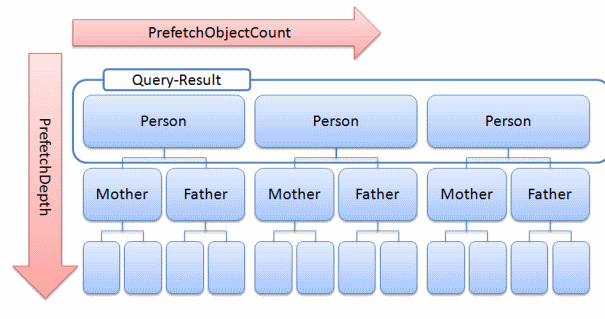
\includegraphics[width=\maxwidth]{images/ref-configuration-client-prefetch-visualisation.png}
\end{center}
\subsection{Prefetch Object Count}
\label{ref:configuration-client-prefetch-object-count}

In a client server scenario, network latency is one of the biggest performance concerns. Instead of making lots of little requests, it's more to do bulk operations. A good way is to prefetch objects which are maybe required later.

The prefect count configures how many objects of a query-result are loaded from the server. Prefetched objects avoid additional roundtrip's to the server for getting the data. However more data needs to be sent to the clients.

\begin{lstlisting}
ClientConfiguration configuration = Db4oClientServer.newClientConfiguration();
configuration.prefetchObjectCount(500);
\end{lstlisting}

{\small\itshape ClientConfigurationExamples.java: Configure the prefetch object count\par}
\medskip

The \hyperref[ref:configuration-client-prefetch-depth]{prefetch depth} (p.~\pageref{ref:configuration-client-prefetch-depth}) and the \hyperref[ref:configuration-client-prefetch-object-count]{prefetch object count} (p.~\pageref{ref:configuration-client-prefetch-object-count}) are closely related to each other. The prefetch object count configures how many objects are prefetched from a query-result. The prefetch-depth configures how deep the object-graph is fetched.

\begin{center}
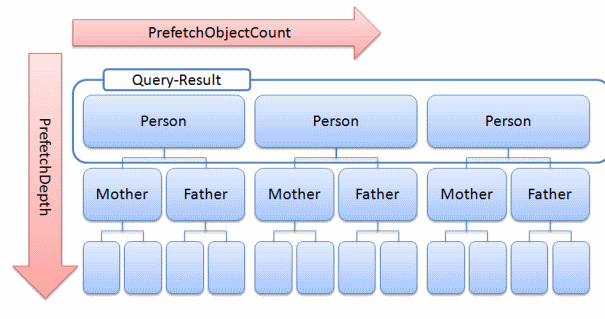
\includegraphics[width=\maxwidth]{images/ref-configuration-client-prefetch-visualisation.png}
\end{center}
\subsection{Prefetch Slot Cache Size}
\label{ref:configuration-client-prefetch-slot-cache-size}

Configures how big the cache for prefetched data is. A larger cache can improve performance, but consumes more memory.

\begin{lstlisting}
ClientConfiguration configuration = Db4oClientServer.newClientConfiguration();
configuration.prefetchSlotCacheSize(1024);
\end{lstlisting}

{\small\itshape ClientConfigurationExamples.java: Configure the slot cache\par}
\medskip

\subsection{Prefetching IDs For New Objects}
\label{ref:configuration-client-prefecht-id-count}

Sets the number of IDs to be pre-allocated new objects created on the client. This avoids requests to allocate new ids when new objects are stored on a client.

When a new object is created on a client, the client should contact the server to get the next available object ID. PrefetchIDCount allows to specify how many IDs should be pre-allocated on the server and prefetched by the client. This method helps to reduce client-server communication.

PrefetchIDCount can be tuned to approximately match the usual amount of objects created in one operation to improve the performance.

When the PrefetchIDCount is one, the client will have to connect to the server for each new objects created. On the other hand,, when the PrefetchIDCount is bigger than the amount of new objects the database will keep unnecessary preallocated ids.

The default PrefetchIDCount is 10.

\subsection{Timeout Client Socket}
\label{ref:configuration-client-timeout-client-socket}

Configure how long it takes, before an inactive connection is timed out.

\begin{lstlisting}
ClientConfiguration configuration = Db4oClientServer.newClientConfiguration();
configuration.timeoutClientSocket(1*60*1000);
\end{lstlisting}

{\small\itshape ClientConfigurationExamples.java: Configure the timeout\par}
\medskip

\section{Networking Configuration}
\label{ref:configuration-network-configuration}

The networking-configuration apply to the client- and the server-mode of db4o. All the networking configuration is accessible via the networking-getter on the configuration-object.

Note that the networking configuration should be the same on the server and all clients.

\subsection*{Overview}

Here's a overview over all networking configuration-settings which you can change:

{\small
\begin{longtable}{|p{\dimexpr(\linewidth-2\arrayrulewidth)*1/1-2\tabcolsep\relax}|}
\hline
\textbf{\hyperref[ref:configuration-networking-batch-mode]{BatchMessages} (p.~\pageref{ref:configuration-networking-batch-mode})}: Enable/Disable batch messages. \\ \hline
\textbf{\hyperref[ref:client-server-messaging]{MessageRecipient} (p.~\pageref{ref:client-server-messaging})}: Set the message receiver. \\ \hline
\textbf{\hyperref[ref:configuration-networking-client-server-factory]{ClientServerFactory} (p.~\pageref{ref:configuration-networking-client-server-factory})}: Replace the client-server factory. \\ \hline
\textbf{\hyperref[ref:configuration-networking-max-batch-queue-size]{MaxBatchQueueSize} (p.~\pageref{ref:configuration-networking-max-batch-queue-size})}: Set the maximum size of the batch queue. \\ \hline
\textbf{\hyperref[ref:configuration-networking-single-threaded-client]{SingleThreadedClient} (p.~\pageref{ref:configuration-networking-single-threaded-client})}: Set the client to single threaded. \\ \hline
\textbf{\hyperref[ref:configuration-networking-pluggable-sockets]{SocketFactory} (p.~\pageref{ref:configuration-networking-pluggable-sockets})}: Set the socket-factory. \\ \hline
\end{longtable}}

\subsection{Batch Mode}
\label{ref:configuration-networking-batch-mode}

Batch mode allows to increase the performance by reducing client/server communication. It's activated by default.

\begin{lstlisting}
ClientConfiguration configuration = Db4oClientServer.newClientConfiguration();
configuration.networking().batchMessages(true);
\end{lstlisting}

{\small\itshape NetworkConfigurationExample.java: enable or disable batch mode\par}
\medskip

db4o communicates with the server by means of messaging. Without batch mode db4o sends a message for each operation and waits for the response. This might be quite inefficient when there are many small messages to be sent (like bulk inserts, updates, deletes). The network communication becomes a bottleneck. Batch messaging mode solves this problem by caching the messages and sending them only when required.

\subsubsection*{Advantages}

\begin{itemize}
\item Reduced network load.
\item Increased performance for bulk operations.
\end{itemize}

\subsubsection*{Disadvantages}

\begin{itemize}
\item Increased memory consumption on both the client and the server. \hyperref[ref:configuration-networking-max-batch-queue-size]{See "Max Batch Queue Size"} (p.~\pageref{ref:configuration-networking-max-batch-queue-size})
\end{itemize}

\subsection{Client Server Factory}
\label{ref:configuration-networking-client-server-factory}

Allows you to change the behavior how a client or a server is created.

This setting should be set to the same value on the server and the clients.

\begin{lstlisting}
ClientConfiguration configuration = Db4oClientServer.newClientConfiguration();
configuration.networking().clientServerFactory(new StandardClientServerFactory());
\end{lstlisting}

{\small\itshape NetworkConfigurationExample.java: exchange the way a client or server is created\par}
\medskip

\subsection{Message Recipient}
\label{ref:configuration-networking-message-recipient}

Register a message recipient for the this object container / server. \hyperref[ref:client-server-messaging]{See "Messaging"} (p.~\pageref{ref:client-server-messaging})

\subsection{Max Batch Queue Size}
\label{ref:configuration-networking-max-batch-queue-size}

To avoid unnecessary network traffic, the client and server can queue up operations, which don't need to be executed immediately. As soon as a message need to be send, all queued messages are send as well. You can configure the maximum of this message queue.

A larger size allows to queue up more messages and avoid unnecessary network roundtrip's. However queued up messages consume additional memory.

\begin{lstlisting}
ClientConfiguration configuration = Db4oClientServer.newClientConfiguration();
configuration.networking().maxBatchQueueSize(1024);
\end{lstlisting}

{\small\itshape NetworkConfigurationExample.java: change the maximum batch queue size\par}
\medskip

\subsection{Single Threaded Client}
\label{ref:configuration-networking-single-threaded-client}

You can configure the client to be single-threaded. When you enable this option, the client doesn't use background threads to handle the client-server communication.

\begin{lstlisting}
ClientConfiguration configuration = Db4oClientServer.newClientConfiguration();
configuration.networking().singleThreadedClient(true);
\end{lstlisting}

{\small\itshape NetworkConfigurationExample.java: single threaded client\par}
\medskip

\subsubsection*{Advantage}

On some smaller embedded systems reducing the running threads improves the performance significantly.

\subsubsection*{Disadvantage}

Since all operations run in a single thread, the operations may take longer. Additionally you cannot receive \hyperref[ref:client-server-messaging]{messages} (p.~\pageref{ref:client-server-messaging}) and cannot use \hyperref[ref:advanced-topics-callbacks-event-registry-api]{commit-callbacks} (p.~\pageref{ref:advanced-topics-callbacks-event-registry-api}) on a single-threaded client.

\subsection{Pluggable Sockets}
\label{ref:configuration-networking-pluggable-sockets}

db4o allows to customize client-server communication by using pluggable socket implementations.

\begin{lstlisting}
ClientConfiguration configuration = Db4oClientServer.newClientConfiguration();
configuration.networking().socketFactory(new StandardSocket4Factory());
\end{lstlisting}

{\small\itshape NetworkConfigurationExample.java: Exchange the socket-factory\par}
\medskip

One use case for changing the socket-implementation is encryption. In fact, db4o's SSL-support uses this mechanism: \hyperref[ref:client-server-pluggable-sockets-using-ssl-for-client-server-communication]{See "Using SSL For Client-Server Communication"} (p.~\pageref{ref:client-server-pluggable-sockets-using-ssl-for-client-server-communication})

\section{Class Specific Configuration}
\label{ref:configuration-objectclass-configuration}

Some settings are object-specific and are configured for the class. It's part of the \hyperref[ref:configuration-common-configuration]{common} (p.~\pageref{ref:configuration-common-configuration})-configuration, which is available on the \hyperref[ref:configuration-client-configuration]{client} (p.~\pageref{ref:configuration-client-configuration}), \hyperref[ref:configuration-server-configuration]{server} (p.~\pageref{ref:configuration-server-configuration}) and \hyperref[ref:configuration]{embedded} (p.~\pageref{ref:configuration})-mode of db4o.

Its recommended that you use the same configuration for the client and the server.

\subsection*{Access the Class Configuration}

The configuration for a specific class follows always the same pattern. First you specify for which type the configuration applies. You pass the type, the name as string or event an instance of the specific class to the configuration.

From the class-configuration, you also can go a level deeper to \hyperref[ref:configuration-objectfield-configuration]{the field configuration} (p.~\pageref{ref:configuration-objectfield-configuration}).

\subsection*{Overview}

Here's a overview over all common configuration-settings which you can change:

{\small
\begin{longtable}{|p{\dimexpr(\linewidth-2\arrayrulewidth)*1/1-2\tabcolsep\relax}|}
\hline
\textbf{\hyperref[ref:configuration-objectclass-call-constructor]{CallConstructor} (p.~\pageref{ref:configuration-objectclass-call-constructor})}: Configure db4o to call constructors when instantiating objects. \\ \hline
\textbf{\hyperref[ref:configuration-objectclass-cascade-on-delete]{CascadeOnDelete} (p.~\pageref{ref:configuration-objectclass-cascade-on-delete})}: When a object is deleted, delete also referenced objects. \\ \hline
\textbf{\hyperref[ref:configuration-objectclass-cascade-on-update]{CascadeOnUpdate} (p.~\pageref{ref:configuration-objectclass-cascade-on-update})}: When a object is updated, update also referenced objects. \\ \hline
\textbf{\hyperref[ref:configuration-objectclass-cascade-on-activate]{CascadeOnActivation} (p.~\pageref{ref:configuration-objectclass-cascade-on-activate})}: When a object is activated, activate also referenced objects. \\ \hline
\textbf{\hyperref[ref:configuration-objectclass-diable-class-index]{Index} (p.~\pageref{ref:configuration-objectclass-diable-class-index})}: Don't index the objects of this type. \\ \hline
\textbf{\sout{EnableReplication}}: Deprecated. \hyperref[ref:configuration-file-generate-uuids]{Generate uuids} (p.~\pageref{ref:configuration-file-generate-uuids}) and \hyperref[ref:configuration-file-generate-timestamps]{commit timestamps} (p.~\pageref{ref:configuration-file-generate-timestamps}) to enable replication. \\ \hline
\textbf{\hyperref[ref:configuration-objectclass-generate-uuid]{GenerateUUIDs} (p.~\pageref{ref:configuration-objectclass-generate-uuid})}: Generate UUIDs, mainly used for replication. \\ \hline
\textbf{\sout{GenerateVersionNumbers}}: Deprecated. Generate \hyperref[ref:configuration-file-generate-timestamps]{commit timestamps} (p.~\pageref{ref:configuration-file-generate-timestamps}) instead. \\ \hline
\textbf{\hyperref[ref:configuration-objectclass-maximum-activation-depth]{MaximumActivationDepth} (p.~\pageref{ref:configuration-objectclass-maximum-activation-depth})}: Set a maximum activation-depth. \\ \hline
\textbf{\hyperref[ref:configuration-objectclass-minimum-activation-depth]{MinimumActivationDeph} (p.~\pageref{ref:configuration-objectclass-minimum-activation-depth})}: Set a minimum activation-depth. \\ \hline
\textbf{\hyperref[ref:configuration-objectclass-persist-static-fields]{PersistStaticFields} (p.~\pageref{ref:configuration-objectclass-persist-static-fields})}: Persist also the static fields of this type. \\ \hline
\textbf{\hyperref[ref:configuration-objectclass-rename-class]{Rename} (p.~\pageref{ref:configuration-objectclass-rename-class})}: Rename this type. Used for \hyperref[ref:advanced-topics-refactoring-and-schema-evolution]{refactorings} (p.~\pageref{ref:advanced-topics-refactoring-and-schema-evolution}). \\ \hline
\textbf{\hyperref[ref:configuration-objectclass-set-a-translator]{Translate} (p.~\pageref{ref:configuration-objectclass-set-a-translator})}: Set a translator for this type. \\ \hline
\textbf{\hyperref[ref:configuration-objectclass-store-transient-fields]{StoreTransientFields} (p.~\pageref{ref:configuration-objectclass-store-transient-fields})}: Store also transient fields. \\ \hline
\textbf{\hyperref[ref:configuration-objectclass-update-depth]{UpdateDepth} (p.~\pageref{ref:configuration-objectclass-update-depth})}: Set the update-depth for this type. \\ \hline
\end{longtable}}

\subsection{Call Constructor}
\label{ref:configuration-objectclass-call-constructor}

By default db4o bypassed the constructor when it loads the objects from the database. When you're class relies on the constructor to be called, for example to initialize transient state, you can enable it. You can do this also on the global configuration for all types. \hyperref[ref:configuration-common-calling-constructors]{See "Calling Constructors"} (p.~\pageref{ref:configuration-common-calling-constructors})

\begin{lstlisting}
EmbeddedConfiguration configuration = Db4oEmbedded.newConfiguration();
configuration.common().objectClass(Person.class).callConstructor(true);
\end{lstlisting}

{\small\itshape ObjectConfigurationExamples.java: Call constructor\par}
\medskip

\subsection{Cascade on Delete}
\label{ref:configuration-objectclass-cascade-on-delete}

When turned on the deletion cascades to all referred objects.

\begin{lstlisting}
EmbeddedConfiguration configuration = Db4oEmbedded.newConfiguration();
configuration.common().objectClass(Person.class).cascadeOnDelete(true);
\end{lstlisting}

{\small\itshape ObjectConfigurationExamples.java: When deleted, delete also all references\par}
\medskip

\subsection{Cascade on Update}
\label{ref:configuration-objectclass-cascade-on-update}

When turned on, the update cascades to all referred objects.

Note: As soon as you use \hyperref[ref:basics-transparent-persistence]{transparent persistence} (p.~\pageref{ref:basics-transparent-persistence}) this configuration option has no effect and isn't needed.

\begin{lstlisting}
EmbeddedConfiguration configuration = Db4oEmbedded.newConfiguration();
configuration.common().objectClass(Person.class).cascadeOnUpdate(true);
\end{lstlisting}

{\small\itshape ObjectConfigurationExamples.java: When updated, update also all references\par}
\medskip

\subsection{Cascade on Activate}
\label{ref:configuration-objectclass-cascade-on-activate}

db4o uses the concept of \hyperref[ref:basics-activation]{activation} (p.~\pageref{ref:basics-activation}) to avoid loading to much data into memory. When turned on the activation cascades for this types. This means that when an instance is activated, all referenced objects are also activated.

Note: As soon as you use \hyperref[ref:basics-transparent-persistence]{transparent activation/persistence} (p.~\pageref{ref:basics-transparent-persistence}) this configuration option has no effect.

\begin{lstlisting}
EmbeddedConfiguration configuration = Db4oEmbedded.newConfiguration();
configuration.common().objectClass(Person.class).cascadeOnActivate(true);
\end{lstlisting}

{\small\itshape ObjectConfigurationExamples.java: When activated, activate also all references\par}
\medskip

\subsection{Disable Class Index}
\label{ref:configuration-objectclass-diable-class-index}

By default there's a index which indexes all instances of a certain type. When you never query this type and only access it by navigation, you can safely disable this index.

\begin{lstlisting}
EmbeddedConfiguration configuration = Db4oEmbedded.newConfiguration();
configuration.common().objectClass(Person.class).indexed(false);
\end{lstlisting}

{\small\itshape ObjectConfigurationExamples.java: Disable class index\par}
\medskip

\subsection{Generate UUIDs}
\label{ref:configuration-objectclass-generate-uuid}

Generate UUIDs for instances of this type. UUIDs are mainly used for \hyperref[drs:welcome]{replication} (p.~\pageref{drs:welcome}).

\begin{lstlisting}
EmbeddedConfiguration configuration = Db4oEmbedded.newConfiguration();
configuration.common().objectClass(Person.class).generateUUIDs(true);
\end{lstlisting}

{\small\itshape ObjectConfigurationExamples.java: Generate uuids for this type\par}
\medskip

\subsection{Maximum Activation Depth}
\label{ref:configuration-objectclass-maximum-activation-depth}

Sets the maximum \hyperref[ref:basics-activation]{activation depth} (p.~\pageref{ref:basics-activation}) for this type. Useful to avoid accidentally activating large objects.

Note: As soon as you use \hyperref[ref:basics-transparent-persistence]{transparent activation/persistence} (p.~\pageref{ref:basics-transparent-persistence}) this configuration option has no effect.

\begin{lstlisting}
EmbeddedConfiguration configuration = Db4oEmbedded.newConfiguration();
configuration.common().objectClass(Person.class).maximumActivationDepth(5);
\end{lstlisting}

{\small\itshape ObjectConfigurationExamples.java: Set maximum activation depth\par}
\medskip

\subsection{Minimum Activation Depth}
\label{ref:configuration-objectclass-minimum-activation-depth}

Sets the minimum \hyperref[ref:basics-activation]{activation depth} (p.~\pageref{ref:basics-activation}) for this type. Useful to load always load referenced objects.

Note: As soon as you use \hyperref[ref:basics-transparent-persistence]{transparent activation/persistence} (p.~\pageref{ref:basics-transparent-persistence}) this configuration option has no effect.

\begin{lstlisting}
EmbeddedConfiguration configuration = Db4oEmbedded.newConfiguration();
configuration.common().objectClass(Person.class).minimumActivationDepth(2);
\end{lstlisting}

{\small\itshape ObjectConfigurationExamples.java: Set minimum activation depth\par}
\medskip

\subsection{Persist Static Fields}
\label{ref:configuration-objectclass-persist-static-fields}

By default db4o doesn't store static fields. With this setting you force db4o to also store the value of the static fields. Note that only reference types are stored. Value-types like ints, longs etc are not persisted.

In general you shouldn't store static fields, because this can lead to unexpected behaviors. It's mostly useful for enumeration classes. \hyperref[ref:advanced-topics-type-handling-static-fields-and-enums-static-fields-api]{See "Storing Static Fields"} (p.~\pageref{ref:advanced-topics-type-handling-static-fields-and-enums-static-fields-api})

\begin{lstlisting}
EmbeddedConfiguration configuration = Db4oEmbedded.newConfiguration();
configuration.common().objectClass(Person.class).persistStaticFieldValues();
\end{lstlisting}

{\small\itshape ObjectConfigurationExamples.java: Persist also the static fields\par}
\medskip

\subsection{Rename Class}
\label{ref:configuration-objectclass-rename-class}

You can rename a class. Useful when you reactor you're code. \hyperref[ref:advanced-topics-refactoring-and-schema-evolution]{See "Refactoring and Schema Evolution"} (p.~\pageref{ref:advanced-topics-refactoring-and-schema-evolution})

\begin{lstlisting}
EmbeddedConfiguration configuration = Db4oEmbedded.newConfiguration();
configuration.common().objectClass(Person.class).rename("com.db4odoc.new.package.NewName");
\end{lstlisting}

{\small\itshape ObjectConfigurationExamples.java: Rename this type\par}
\medskip

\subsection{Set a Translator}
\label{ref:configuration-objectclass-set-a-translator}

You can specify a special translator for this type. A translator is a special way to add you're custom serialization for a type. \hyperref[ref:advanced-topics-type-handling-translators]{See "Translators"} (p.~\pageref{ref:advanced-topics-type-handling-translators})

\begin{lstlisting}
EmbeddedConfiguration configuration = Db4oEmbedded.newConfiguration();
configuration.common().objectClass(Person.class).translate(new TSerializable());
\end{lstlisting}

{\small\itshape ObjectConfigurationExamples.java: Use a translator for this type\par}
\medskip

\subsection{Store Transient Fields}
\label{ref:configuration-objectclass-store-transient-fields}

By default db4o doesn't store transient fields. With this setting you can force db4o to event store transient fields.

\begin{lstlisting}
EmbeddedConfiguration configuration = Db4oEmbedded.newConfiguration();
configuration.common().objectClass(Person.class).storeTransientFields(true);
\end{lstlisting}

{\small\itshape ObjectConfigurationExamples.java: Store also transient fields\par}
\medskip

\subsection{Update Depth}
\label{ref:configuration-objectclass-update-depth}

By default db4o only stores changes on the updated object, but not the changes on referenced objects. With a higher update-depth db4o will traverse along the object graph to a certain depth and update all objects. \hyperref[ref:basics-update-concept]{See "Update Concept"} (p.~\pageref{ref:basics-update-concept}). You can also specify this \hyperref[ref:configuration-common-update-depth]{globally} (p.~\pageref{ref:configuration-common-update-depth}).

\begin{lstlisting}
EmbeddedConfiguration configuration = Db4oEmbedded.newConfiguration();
configuration.common().objectClass(Person.class).updateDepth(2);
\end{lstlisting}

{\small\itshape ObjectConfigurationExamples.java: Set the update depth\par}
\medskip

\section{Field Specific Configuration}
\label{ref:configuration-objectfield-configuration}

Some settings are field-specific. It's part of the \hyperref[ref:configuration-objectclass-configuration]{object} (p.~\pageref{ref:configuration-objectclass-configuration})-configuration, which is available on the client, server and embedded-mode of db4o.

Its recommended that you use the same configuration for the client and the server.

\subsection*{Access the Field Configuration}

The configuration for a field follows the same pattern. First you specify for which type this configuration applies. You pass the type or the name as string. Then you navigate to the specific field by passing the field name as string.

\subsection{Adding a Field Index}
\label{ref:configuration-objectfield-configuration:adding}

Index dramatically speed up queries. You should index all fields which you run queries on. \hyperref[ref:basics-indexing]{See "Indexing"} (p.~\pageref{ref:basics-indexing})

\begin{lstlisting}
@Indexed
private String zipCode;
\end{lstlisting}

{\small\itshape City.java: Index a field\par}
\medskip

As alternative you can externally configure a field index:

\begin{lstlisting}
EmbeddedConfiguration configuration = Db4oEmbedded.newConfiguration();
configuration.common().objectClass(Person.class).objectField("name").indexed(true);
\end{lstlisting}

{\small\itshape ObjectFieldConfigurations.java: Index a certain field\par}
\medskip

As an alternative you also can use the appropriate Annotation on the field which you want to index.

\subsection{Cascade On Activate}
\label{ref:configuration-objectfield-configuration:cascadeactivate}

db4o uses the concept of \hyperref[ref:basics-activation]{activation} (p.~\pageref{ref:basics-activation}) to avoid loading to much data into memory. When this setting is turned on, the object referenced by this field is activated, when the object is activated.

Note: As soon as you use \hyperref[ref:basics-transparent-persistence]{transparent activation/persistence} (p.~\pageref{ref:basics-transparent-persistence}) this configuration option has no effect.

\begin{lstlisting}
EmbeddedConfiguration configuration = Db4oEmbedded.newConfiguration();
configuration.common().objectClass(Person.class).objectField("father").cascadeOnActivate(true);
\end{lstlisting}

{\small\itshape ObjectFieldConfigurations.java: When activated, activate also the object referenced by this field\par}
\medskip

\subsection{Cascade On Update}
\label{ref:configuration-objectfield-configuration:cascadeupdate}

When the object is updated, the object referenced by this field is also updated.

Note: As soon as you use \hyperref[ref:basics-transparent-persistence]{transparent persistence} (p.~\pageref{ref:basics-transparent-persistence}) this configuration option has no effect and isn't needed.

\begin{lstlisting}
EmbeddedConfiguration configuration = Db4oEmbedded.newConfiguration();
configuration.common().objectClass(Person.class).objectField("father").cascadeOnUpdate(true);
\end{lstlisting}

{\small\itshape ObjectFieldConfigurations.java: When updated, update also the object referenced by this field\par}
\medskip

\subsection{Cascade On Delete}
\label{ref:configuration-objectfield-configuration:cascadedelete}

When the object is deleted, the object referenced by this field is also deleted

\begin{lstlisting}
EmbeddedConfiguration configuration = Db4oEmbedded.newConfiguration();
configuration.common().objectClass(Person.class).objectField("father").cascadeOnDelete(true);
\end{lstlisting}

{\small\itshape ObjectFieldConfigurations.java: When deleted, delete also the object referenced by this field\par}
\medskip

\subsection{Rename Field}
\label{ref:configuration-objectfield-configuration:rename}

Allows you to rename this field. . \hyperref[ref:advanced-topics-refactoring-and-schema-evolution]{See "Refactoring and Schema Evolution"} (p.~\pageref{ref:advanced-topics-refactoring-and-schema-evolution})

\begin{lstlisting}
EmbeddedConfiguration configuration = Db4oEmbedded.newConfiguration();
configuration.common().objectClass(Person.class).objectField("name").rename("sirname");
\end{lstlisting}

{\small\itshape ObjectFieldConfigurations.java: Rename this field\par}
\medskip

\section{Id System}
\label{ref:configuration-id-system}

The id-system configuration applies to the embedded- and the server-mode of db4o. There are tree different id-systems-available. All the id system configuration is accessible via the id-system-getter on the configuration-object.

Note that you cannot change the id-system for an existing database. You need to \hyperref[ref:advanced-topics-defragment]{defragment} (p.~\pageref{ref:advanced-topics-defragment}) the database in order to change the id-system.

The id-system is responsible to mapping a object id to the physical location of an object. This mapping can have significant impact on the performance.

\subsection*{Stacked BTree Id-System}

This setting uses a stack of two BTree's on top of an InMemoryIdSystem. This system is scalable for a large number of ids.

\begin{lstlisting}
EmbeddedConfiguration configuration = Db4oEmbedded.newConfiguration();
configuration.idSystem().useStackedBTreeSystem();
\end{lstlisting}

{\small\itshape IdSystemConfigurationExamples.java: Use stacked B-trees for storing the ids\par}
\medskip

\subsection*{Single BTree Id-System}

This setting uses a single BTree on top of a in memory id system. This system works great for small databases. However it cannot scale for a large number of ids.

\begin{lstlisting}
EmbeddedConfiguration configuration = Db4oEmbedded.newConfiguration();
configuration.idSystem().useSingleBTreeSystem();
\end{lstlisting}

{\small\itshape IdSystemConfigurationExamples.java: Use a single B-tree for storing the ids.\par}
\medskip

\subsection*{In Memory Id-System}

This id-system keeps all ids in memory. While accessing the ids if fast, all ids have to be written to disk on every commit. Therefore it can be used only for tiny databases.

\begin{lstlisting}
EmbeddedConfiguration configuration = Db4oEmbedded.newConfiguration();
configuration.idSystem().useInMemorySystem();
\end{lstlisting}

{\small\itshape IdSystemConfigurationExamples.java: Use a in-memory id system\par}
\medskip

\subsection*{Pointer Based Id-System}

This id system uses pointers to handle ids. Each id represents a pointer into the database-file. This makes the id-mapping simple. However since it's a pointer, you cannot change the location. Therefore this system leads to more fragmentation and performance degradation as the database grows.

This id system is here to ensure backward-compatibility. It's not recommended to use for new databases.

\begin{lstlisting}
EmbeddedConfiguration configuration = Db4oEmbedded.newConfiguration();
configuration.idSystem().usePointerBasedSystem();
\end{lstlisting}

{\small\itshape IdSystemConfigurationExamples.java: Use pointers for storing the ids\par}
\medskip

\subsection*{Custom Id-System}

It's possible to implement your own id system. You can pass an factory which creates your id-system implementation.

\begin{lstlisting}
EmbeddedConfiguration configuration = Db4oEmbedded.newConfiguration();
configuration.idSystem().useCustomSystem(new CustomIdSystemFactory());
\end{lstlisting}

{\small\itshape IdSystemConfigurationExamples.java: use a custom id system\par}
\medskip

\section{Server Configuration}
\label{ref:configuration-server-configuration}

The server-configuration applies to the \hyperref[ref:client-server]{db4o-server} (p.~\pageref{ref:client-server}). All the server specific configuration is directly on the client configuration interface.

You can also configure the \hyperref[ref:configuration-common-configuration]{common} (p.~\pageref{ref:configuration-common-configuration})-, \hyperref[ref:configuration-file-configuration]{file} (p.~\pageref{ref:configuration-file-configuration})-, \hyperref[ref:configuration-id-system]{id-system} (p.~\pageref{ref:configuration-id-system})- and the \hyperref[ref:configuration-network-configuration]{network} (p.~\pageref{ref:configuration-network-configuration})-settings for a server.

\subsection*{Server Socket Timeout}

Configure how long it takes, before an inactive connection is timed out.

\begin{lstlisting}
ServerConfiguration configuration = Db4oClientServer.newServerConfiguration();
configuration.timeoutServerSocket(10*60*1000);
\end{lstlisting}

{\small\itshape ServerConfigurationExamples.java: configure the socket-timeout\par}
\medskip

